\documentclass{report}
\usepackage[a4paper, margin=1.5in]{geometry}
\setlength{\parindent}{0em}
\setlength{\parskip}{1.2em}
\renewcommand{\baselinestretch}{1.3}
\usepackage[utf8]{inputenc}
\usepackage{graphicx}
\usepackage{tabularx}
\usepackage{amsmath}
\usepackage{amssymb}
\usepackage{listings}
\usepackage{makecell}
\usepackage{longtable}
\usepackage{pdfpages}

\title{An Attempt to Use Machine Learning to Classify Novice and Expert Developers}
\author{
    Lee Chi Hong\\
    BSc Hons Computer Science\\
    Lancaster University
}
\date{19 March 2021}

\begin{document}

\maketitle

\pagenumbering{roman}

\addcontentsline{toc}{section}{Declaration of Originality}
\begin{center}
    \textbf{Declaration of Originality}
\end{center}
I certify that the material contained in this dissertation is my own work and does not contain unreferenced or unacknowledged material. I also warrant that the above statement applies to the implementation of the project and all associated documentation. Regarding the electronically submitted work, I consent to this being stored electronically and copied for assessment purposes, including the School’s use of plagiarism detection systems in order to check the integrity of assessed work.

I agree to my dissertation being placed in the public domain, with my name explicitly included as the author of the work.

Name: Lee Chi Hong\\
Date: 19 March 2021

\newpage

\addcontentsline{toc}{section}{Abstract}
\begin{center}
    \textbf{Abstract}
\end{center}
This project aims to distinguish novice and expert developers using machine learning. This is important and beneficial in different cases, such as higher education institutions providing computer science courses, companies hiring developers or developers hoping to evaluate their experience level. In the first part of the project, a variety of different models were trained with different data gathered from novice and expert, to identify the best model and data combination for this purpose. The final model is able to achieve a 69.0\% accuracy. Features extraction mainly focused on static code analysis. In the later part, two application prototypes were developed using the stated model for two different use case scenarios which require experience classification of developers.

A repository containing all data collected, source code of scripts and applications developed for this project can be found at: https://gabrielchl.dev/2021-thesis-repo

\addcontentsline{toc}{section}{Acknowledgements}
\begin{center}
    \textbf{Acknowledgements}
\end{center}
Special thanks to Professor Tracy Hall, the supervisor for this project for her guidance, feedback and support throughout the project.

\newpage

\pagenumbering{arabic}

\setlength{\parskip}{0.5em}
\tableofcontents
\setlength{\parskip}{1.2em}

\chapter{Introduction}

Code stylometry is a type of stylometry for binary or source code. It is the study of program authorship or related analysis through feature identification in code. This has numerous benefits, such as giving us the ability to identify possible code plagiarism and to identify the source of malicious software. Many research studies have been conducted in this field, with at least 57 publications published between 1957 and 2020 related to this topic (Kalgutkar et al., 2019).

The vast majority of the research mentioned above focuses on attributing the author of a piece of code, very few research studies were done to classify properties of the author of pieces of code, such as the author’s level of experience in coding. Thus, the main aim of this project is to explore the approach of using machine learning with code stylometry for such classification problem. While a successful project, that is to be able to obtain a highly accurate model for the problem, is not guaranteed, this project aims to offer valuable insight and data from using the techniques mentioned above.

\section{Project Importance}

The ability to classify developers as novice or expert could bring positive impact in a vast amount of scenarios, as we explore below.

For individual developers, knowing their skill level compared to their peers is a very useful tool in their learning progress. Such self-awareness helps individuals to know where they are standing on the path to being an expert in the computer science field. In Loksa D. et al. (2016)’s study, they studied the impact of several teaching techniques on students learning to code. Results show that the four techniques, one of them being prompting those students to reflect on the problem solving strategies they have used, results in increased productivity, self-efficacy and brings positive impact to the students’ growth mindset. Patricia S. (2014)’s article states that without self-awareness, we could not accurately identify our strengths and weaknesses, which is very important in the lifelong learning process.

For higher education institutions, this ability is the key to providing an accurately-tailored educational experience for students with a wide range of skill levels in programming. There has been a lot of research on different education techniques, that all require the classification of stronger and weaker students. Agrawal et al. (2014)’s study shows that grouping strong students with weaker students could maximize the number of students doing better. Lui et al. (2014)’s study shows that using a “Perform” teaching approach would help weak students achieve better performance. Their research targeted weak programmer students in their first programming course, by isolating weak students and “shielding” them from certain “hazards” under the Perform teaching approach, they were more able to write simple programs, achieve higher performance in the examination and improve confidence in programming. These researches highlight the importance of the ability to classify students by their strength. With the model that this project develops, teachers and professors will be able to quickly do so.

For companies hiring programmers, it is proven that companies are very likely to exclude exceptional candidates if students’ GPA was used to pre-screen or filter the candidates (Clark et al., 2003). The ability to distinguish experienced developers to novices allows them to gain insight into any candidates quickly and accurately, improving their hiring process. A minor benefit of such ability is to help identify fraudulent applications. According to a survey of 1000 UK citizens, 38\% have lied at least once on their CV, with 24\% doing so regularly (Job Today, 2017). Employing candidates who exaggerate or falsify certain information on their CV could cost the company both monetary and legally (Babcock, 2003). With the ability to determine if a developer is a novice or expert, this could help companies identify inconsistency between candidates’ real experience and what is stated on their job application.

\section{Project Overview}

This project is designed to be separated into two distinct parts, model training and application development, with the model training part given a higher priority.

For the model training part, a mathematical model was developed using data from novice and expert developers. These data were crawled from HackerRank, a competitive programming or programming interview preparation site. Different configurations to fetch such data and features to extract were experimented to optimize the model accuracy. The final model is able to achieve a 68\% accuracy.

For the application development part, two applications were developed, one as a website application and the other as a desktop application. These two applications were developed as a prototype, to demonstrate possible uses of the model trained in the first part of the project. The website application was designed for individual developer’s use, while the desktop application was designed for corporate or institution’s use.

\section{Project Aims}

The overall target of this project is to explore the possibility and if so, to contribute data to establish code author attributes through the use of machine learning models. The project can be broken down into the following list of objectives.

\begin{enumerate}
\item Determine if it is possible to classify developers’ experience level using features from their code
\item Determine what features would be helpful for the model
\item Determine what model would help achieve better classification accuracy
\item Develop one or more prototype applications to demonstrate possible uses of such model
\end{enumerate}

\section{Report Overview}

The rest of the report is broken down into the following various sections.

In Chapter 2 “Background Research”, previous research into code stylometry, machine learning, developers’ coding experience and application design and development is introduced and summarized. Useful information that helps this project is highlighted from those research.

In Chapter 3 “Machine Learning Model”, the data source, features extracted, the model used and analysis of the final trained model is introduced. Different experiments on these factors, and certain decisions made throughout the process of attempting to obtain a good model as defined in the project aims are discussed.

In Chapter 4 “Prototype Application”, the two developed prototype applications are introduced. Design decisions, detailed implementation methods are discussed, as are the user's evaluation results and discussion around potential advantages and disadvantages of such applications.

Last but not the least, in Chapter 5 “Discussions and Conclusion”, the list of project aims are reviewed. Limitations of this project, possible future works and final remarks are included.

\chapter{Background}

\section{Code Stylometry}

Stylometry is the study of the style of a piece of text or art. Where, as a member of the stylometry family, code stylometry focuses on a piece of code. Code stylometry is used for software forensics, which is the determination of if intellectual property rights were infringed, plagiarism detection, authorship attribution, which is the identification of the author and is what most research on code stylometry focuses on, and authorship analysis, which is the analysis of certain properties of the author.

Code stylometry has been applied to a huge range of different code, including different programming languages, both in source code format or binary code. In most cases, to study the style of a piece of code, certain features in the code would be analysed. This is similar to using text features in linguistic stylometry, or linguistic forensics, techniques, such as the number of words, number of different words, vocabulary richness, grammar mistakes, et cetera (Guillen-Nieto et al., 2008). A lot of research has been conducted to explore the application of linguistic features and features specific to programming languages or binary code on code stylometry.

Halstead (1977) proposed a set of metrics to evaluate a piece of code. Instead of using metrics that depend on or could be affected by the machine it is run on, he proposed a set of features, later called Halstead Metrics, that measures the complexity of the code, which is heavily affected by the algorithms used in the code. As one of the earliest sets of metrics proposed to objectively evaluate code, it has been widely used to analyze code for various uses. In one case, it was one of the sets of metrics found to have strong correlations with computer programming courses’ students’ performance (Castellanos et al., 2017). Halstead’s metrics was also found suitable to use for software defect prediction (Mori and Uchihira, 2018).

In one of the earlier papers on code authorship attribution, Oman and Cook (1989) used a set of metrics inspired by the techniques used for English literature authorship analysis. The set of 16 code characteristics used are as below, where the names of the characteristics are directly from Oman and Cook and the grouping of the characteristics is similar to that of their findings after the protocols studies:

\begin{itemize}
\item Comments
\begin{itemize}
\item Inline comments on the same line as source code
\item Blocked comments (two or more comments occurring together)
\item Bordered comments (set off by repetitive characters)
\item Keywords followed by comments
\end{itemize}
\item Indentation
\begin{itemize}
\item 1 or 2 space indentation most frequently occurring
\item 3 or 4 space indentation most frequently occurring
\item 5 or greater indentation most frequently occurring
\end{itemize}
\item Letter case
\begin{itemize}
\item Lower case characters only (all source code)
\item Upper case characters only (all source code)
\end{itemize}
\item Identifiers
\begin{itemize}
\item Case used to distinguish between keywords and identifiers
\item Underscore used in identifiers
\end{itemize}
\item Statements
\begin{itemize}
\item BEGIN followed by a statement on the same line
\item THEN followed by a statement on the same line
\item Multiple statements per line
\end{itemize}
\item Blank lines
\begin{itemize}
\item Blank lines in the declaration area
\item Blank lines in the program body
\end{itemize}
\end{itemize}

Each of the metrics would give a boolean value. The authors then got 3 PASCAL code snippets, bubble sort, quick sort and tree traversal solutions, from each of the 6 computer science textbooks by different authors. Applying cluster analysis on the metric of code snippet to the 16 boolean values, the authors found 4 of the author’s codes showing a perfect or very high connection level. They then repeated the same procedure on 3 companies’ code, each split into 6 modules, and found 2 of them clustering together perfectly, while for the third company, the modules shared a lower level of similarity, but 5 of the 6 modules were still clustered correctly.

Criticizing that prior studies, including that by Oman and Cook, were “limited in scope and focus, Spafford and Weeber (1993) discussed the difficulties and approaches to analyzing code left in a computer system by a hacker to establish his or her identity. They proposed a longer list of possible types of features to be analyzed for source code or binary code files, where those feature types focusing on source code analysis includes:

\begin{itemize}
\item Language (The programming language used)
\item Formatting (Number of statements per line, type and function declarator formatting, et cetera)
\item Special features (Such as code specific for certain compilers to read)
\item Comments (Consistency, frequency and length)
\item Variable names (Variable name formatting, naming styles of local temporary variables)
\item Language features (Usage of for loops versus while loops, data types, size of modules, et cetera)
\item Scoping (Global versus local identifiers, scope of helper functions)
\item Errors
\item Other metrics (Halstead metrics, McCabe metrics, et cetera)
\end{itemize}

Another type of features that were explored were n-grams. Burrows and Tahaghoghi (2007) explored the use of n-grams for code authorship analysis. Firstly, with 10 authors and 16 C code files, they found 6-gram to be the best performer in 1 to 90-grams, having a 77.77\% accuracy. Next, they investigated the effect of increasing the code source pool to accuracy. With 1640 files from 100 authors, they maintained a 67.01\% accuracy. A more recent study also utilising n-grams by Wisse and Veenman (2015) combined 10 traditional structural, style and layout features with 4 different n-gram metrics to reach a 91.4\% accuracy with 10 authors and 85\% accuracy with 45 authors. In their study, using JavaScript repositories on GitHub, they also compared the accuracy with the same set of metrics but without the 4 n-grams metrics and results seems to indicate the addition of the n-gram metrics does lead to a distinct improvement, especially when the number of training samples is low.

Bhattathiripad (2012) proposes a different type of metrics, programming blunders, to be used to evaluate code. Pointing out that most explored code features focus on the general coding styles or algorithmic choices of the whole piece of code, Bhattathiripad explores the usage of programming blunders to identify code authorship. Examples of programming blunders include unused variables, unused imported libraries, or a section of code that never gets executed. He then proposes the incorporation of such metrics into the US judiciary official software copyright infringement investigation procedure.

With all the different techniques to extract different information and to use different methods to use such information to establish the code author’s identity, there is one flaw, which is the possibility of one imitating another code style to confuse any efforts of code stylometry. Simko et al. (2018) recognizes this issue and observed C and C++ developers obfusticate their own coding styles and the impact on existing machine classifiers and human analysts. Results show that when against machine classifiers, for 80\% of the “attacks”, the developers successfully confused the classifiers. When against human analysts, the author identification accuracy dropped from 92.7\% to 76.2\%. Analyzing the changes those programmers made to confuse machine classifiers, the team pointed out that instead of focusing on local implementation details, such as variable naming styles which could be easily changed, focusing on the algorithmic decisions related metrics, such as complex abstract syntax tree features, would help defend against such attacks.

\section{Code Stylometry with Machine Learning}

While about half of the mentioned research studies in Section 2.1 were only discussions and proposals of techniques, mainly on feature extraction, for code stylometry, the other half applied those techniques with machine learning models on different datasets to perform code author attribution or analysis.

\subsection{Datasets}

There are 3 main types of dataset source used in recent papers.

Private code sources from individuals, organizations or companies. This is usually used when the researches require a very specific type of code or developer. Such as in the case of Hayes and Offutt’s (2010) study, the team wanted to investigate whether developers are always consistent in their coding styles or if they get more consistent as they grow in experience and competency. For this purpose, they had to collect code from very specific groups of developers, 15 graduate students and 5 experienced developers.

Publicly available code repositories on websites such as SourceForge and GitHub. These sources are mostly suitable when a huge number of data is needed as it takes a lot less time than recruiting participants to write or submit code.

Published pieces of code from websites such as Google Code Jam. Google Code Jam is an annual online coding competition where competitors compete to solve programming tasks. (Google Code Jam, 2021) Similar to code repositories on websites, code from these types of websites are usually shorter. Where code repositories usually contain code written for an entire program, these sites provide relatively short scripts. It is also very commonly used in code stylometry related researches (Caliskan-Islam et al., 2015) (Alsulami et al., 2017) (Simko et al., 2018).

\subsection{Classifiers}

Over all the research, a very wide range of machine learning or classifying techniques have been employed.

As mentioned, Oman and Cook (1989) extracted a matrix of boolean values from the code files. They Used SPSS-X cluster analysis to measure the similarity between files to cluster them together and create groups of similar files, from the same author or company.

Zhang et al. (2017) performed code authorship attribution on a very large scale, in one test, with 8000 Java programs from 8 developers, using the sequential minimal optimization algorithm, originally proposed by Platt (1998), to lower the training time required when using support vector machine models. The sequential minimal optimization algorithm is widely used in the community, given its popularity due to the advantages it offers.

Shevertalov et al. (2009) analyzed 60 Java projects by 20 developers, 3 projects from each developer, but with only 4 features extracted: number of leading spaces, number of leading tabs, number of words on each line and the length of each line. They used the nearest neighbour classification method and achieved a 54.3\% and a 75.0\% accuracy on identifying the developers of files and projects respectively. Their study focuses on using genetic algorithm to perform data discretization on the features extracted. The team extracted the four features in the form of a histogram, using genetic algorithm, they identified ideal breakpoints for each column in the histogram, which quite significantly improved the accuracy of the nearest neighbour model. Without data discretization, the accuracy was at 46.1\% and 65\% on the files and projects respectively, around a 10% drop.

Krsul and Spafford (1997) performed a comparison between different machine learning models on identifying the authors of 88 C programs by 29 students. The team extracted 49 features including number of lines, average function parameter length, percentage of lines with inline comments, usage of comment highlighting with borders, et cetera. They then evaluated the performance of multilayer perceptron neural network, gaussian classifier, learning vector qualifier (nearest neighbour), histogram and binary tree classifier. The team was able to reach a 98\% accuracy with neural network and 100\% with Gaussian classifier. This study also revealed the value of normalization with linear discriminant analysis, which helped improve the accuracy by 26\% for the neural network model and 25\% for the Gaussian classifier model.

\section{Experience Classification}

As different individual developers would have different coding styles, the differences in people with different levels of coding experience were also the subject of research papers. These differences could help identify useful features to classify authors of code as a novice or expert.

Wiedenbeck (1985) studied the differences in novice and expert’s programming skills. She measured the accuracy and reaction time of the 2 groups of programmers in two experiments, first when asked to determine if a line of code is syntactically correct or contained an error, and second when asked to determine if a description of a piece of code is accurate. Results from the experiments showed that while the accuracy of novice developers was only 5 - 6\% lower than that of the experts, the experts had a much quicker reaction time.

Counsell et al. (2006) investigated the difference in novice and expert developer’s definition of software cohesion in object-oriented C++ classes. The results show that, while determining the cohesiveness of classes, novice developers are more affected by the number of methods in a class and expert developers are more affected by how well-documented those classes were. This could hint at a different priority in code evaluation, and possibly in writing code.

\chapter{Machine Learning Model}

In this chapter, different processes leading to the creation of the final machine learning model will be discussed. Results and decisions made in key experiments during this process will be reviewed as well.

There is one core principle considered when making any decisions in this part, which is to keep things simple. Given the time, experience and resource limitation, it was decided that the target is to create a simple but working, defined as achieving an accuracy higher than 50\%, model. An example of such principal affecting decisions is when it was being considered whether developers should be categorized into more than 2 categories, novice and expert. With the principle in mind, it was decided to use binary classification, instead of multiple categories or a regression output, to “keep things simple”.

For this project, it was decided that a machine learning model would be developed to predict whether a developer is a novice or expert by analyzing a piece of the developer’s program’s source code.

\section{Data Collection}

To train a machine learning model, data collection is one of the most important steps in the process of developing the model. “Garbage in, garbage out”, this concept is also true for machine learning (Jha et al., 2019), thus this part was carefully planned and carried out.

For this project, there are several criteria for the dataset to be used. Firstly, it should contain code samples from two distinguishable types of developers, novice or experts. Secondly, all code samples should have a certain level of differences, to cover more different developer coding styles. Thirdly, for each type of developer, the number of samples should be reasonable for being used for training a machine learning model. Finally, each code sample should be a one-file script, as to keep the project simple, it was decided not to use entire code repositories or multiple-file programs as the unit of an entry.

Multiple research studies in the past have constructed a dataset for their machine learning model to train on, some of which published their dataset along with their study results. However, as most of such datasets are not focused on differentiating developer experience, they do not contain such classification data, and therefore could not be used for this project. As a result, it was decided to construct a new set of data for the project.

\subsection{Source of Data}

As mentioned in the background section of this report, there are 3 main types of data source, private code sources, code repositories or published code from coding events or competitions. As the project requires a significant amount of data, with limited time available, the first option, private code sources which require lengthy communication and code collection process from participants, is not viable. Hoping to get single-file scripts instead of entire code repositories, coding events or competitions was chosen as the source of data.

There are multiple coding events or competitions that publish participants’ code. While Google Code Jam is a very popular source in related research, it is not suitable to be used in this project as only the username of the participant is available to the public. With the username as the only information from the participant, it is impossible to establish the level of coding experience of that person.

HackerRank is chosen as the data source for this project after evaluations of the website show that its data satisfies the criteria laid and is suitable for this project. HackerRank is a company that provides developer hiring solutions to technology companies by using their coding test systems (HackerRank, 2021). Their website provides coding test practice questions, with over 1 million developers using the website in 2015. The platform has a list of common software engineer interview coding questions, where developers would attempt to solve them and get automated score feedback by running their code and comparing the results to the correct answers. All submitted code is visible to the public, along with the developer’s profile, where some would make use of a feature provided by the website to show a link to their LinkedIn profile. Figure 1 shows a screenshot of the leaderboard of a coding question on the site, allowing access to the users’ profile, shown in Figure 2, to get their LinkedIn profile. With this feature, it is possible to determine if one is a novice or expert developer using the information found on their LinkedIn profile.

\begin{figure}[h!]
\centering
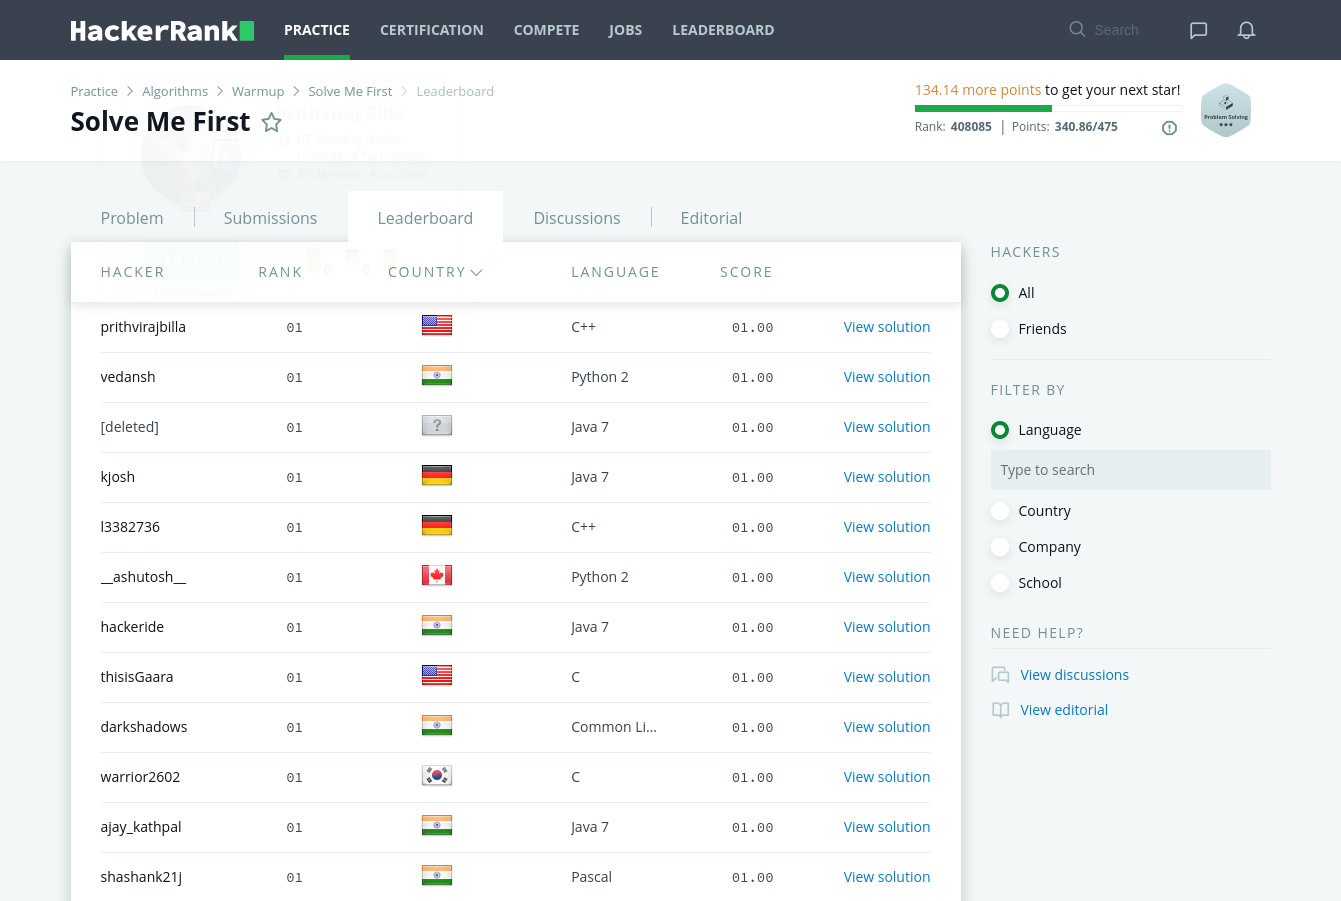
\includegraphics[width=0.8\textwidth]{figure3.1.png}
\caption{Screenshot of a leaderboard page on HackerRank}
\end{figure}

\begin{figure}[h!]
\centering
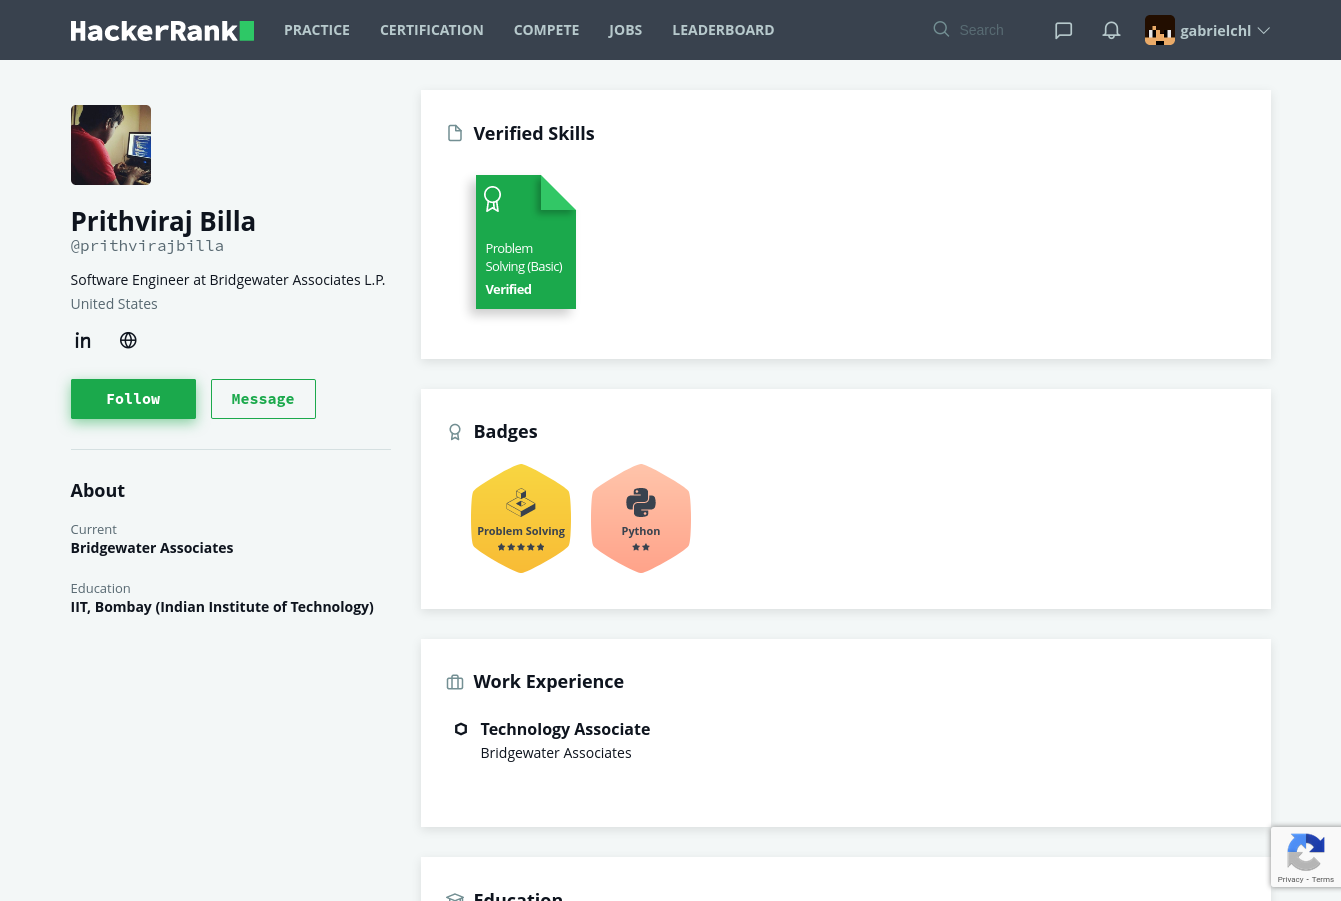
\includegraphics[width=0.8\textwidth]{figure3.2.png}
\caption{Screenshot of a developer’s profile on HackerRank}
\end{figure}

Internal discussions were made on whether using code repositories or HackerRank would be more suitable for this project. Code repositories tend to include more practical code as used in “real life” scenarios, while HackerRank’s code would be more precise and uniform. Using HackerRank’s code, the final model would perform better against competitive programming tasks, but not against general code. Eventually, it was decided that instead of having a generalized but less accurate model, it was more desirable to have a more specific and more accurate model. And therefore HackerRank was selected.

\subsection{Data Extraction}

As a lot of different experiments were carried out for this project, the exact method used for data extraction from HackerRank may differ between some experiments. In this section, the general method would be described, while certain special cases would be mentioned in relevant sections.

Firstly, one or more coding questions would be selected, which will be the source of users’ solution collection. There are 3 main criteria for choosing a question. Firstly, the question should have a reasonable amount of solution submissions, allowing enough instances for the dataset. Secondly, the solutions should show that the question is solvable using different approaches, this helps increase the variety in the features extracted, improving the model’s performance, as proved by Therrien and Doyle (2018). Finally, the question should not be too complicated to be solved by a novice. This is to prevent only collecting experts’ solutions, causing insufficient novice data or an imbalance in the data. This criterion is ensured by using the website’s question difficulty indicator as a reference. Questions marked as “hard” would not be selected.

The next step is to collect the code solutions. As mentioned, from the question’s leaderboard page, it is possible to look up all solutions and their solver. There are a few criteria for the selection of solutions. Firstly, all solutions should be of the same programming language. The site allows submission in a wide range of languages, to produce a simple and precise model, all code samples should be of the same language. For this project, Java was chosen as it is one of the most used languages on the site in terms of the number of submissions using Java. Secondly, all solutions should be using the same code template. When a user starts working on a coding problem, the site would provide a code template, so that the user could focus on the solution instead of the redundant tasks that are the same for each question, such as accepting input from standard input. However, HackerRank occasionally updates those templates, causing fundamental differences in the solutions. For this project, it is decided to filter solutions by only using those with the latest template. Thirdly, only solutions which author’s account is linked to his or her LinkedIn account. Fourthly, the solution should appear as a completed solution, instead of a work in progress or test solution. Finally, the information stated in the LinkedIn profile should satisfy requirements for data labelling, which will be discussed in the next section, data labelling.

For the first few experiments, all solutions were inspected, checking that the solution satisfies the above criteria and that for data labelling, and added to the dataset manually. This was done to ensure a better understanding of those code, which led to some changes to the initial list of the criteria set for the code samples. For later experiments, the solution selection part was automated, with human assistance required to determine if the developer’s LinkedIn profile satisfies the last criteria stated above.

The solution selection automation part was not simple as HackerRank does not provide any publicly available APIs for such uses. The website also has some measures employed to prevent certain bots to traverse the site. To avoid spending much time to offset those measures, instead of writing a script to act as a browser traversing the site, it was opted to make use of browser userscripts. A browser userscript was written using the Violentmonkey plugin for Mozilla firefox (Violentmonkey, 2021). The script goes through the leaderboard and produces a list of users whose solution satisfies the first 4 criteria for the solutions to be selected. The list is then manually inspected, removing entries that do not satisfy the fifth criterion, producing a final list of users whose solution satisfies all criteria.

\subsection{Data Labelling}

Except for certain experiments where the definition of novice and expert was experimented on, which will be covered at the end of this subsection, all experiments share the same definition. The main principle is that whether one does or does not have work experience in development work defines if he or she is a novice or expert.

Before labelling the data, one final check of the validity of the LinkedIn profile was carried out. Profiles with insufficient information, such as the lack of education history or a number of years not accounted for after graduation from a degree, was removed. This prevents mislabelling data due to a lack of information or profiles being not up to date. Any profiles that the experience level could not be determined with confidence was also removed.

For one to be classified as a novice developer, he or she should not have any work experience, including internships or part-time jobs. The user should be studying towards or have graduated from a programming-related degree. For one to be classified as an expert developer, he or she should have any amount of full-time work experience, working at a programming-related position.

Note that experiment 2 is an exception to the above novice and expert definition. In experiment 2, the definition for an expert is if one has at least 6 months of experience on a full-time job, while that for novice developer is if one wrote the piece of code at least 6 months before his or her first job or internship. At the end of the experiment, it was decided to not use this set of definitions as it does not seem to bring significant advantages to the accuracy of the model but increases the time needed to prepare the dataset.

\section{Features Extraction}

\subsection{Features}

Before discussing the final list of features, certain experiments ran to test different combinations of such features shall be mentioned. The very first list of 12 features, being very similar to the final list, included: 1) number of lines 2) number of empty lines 3) number of line comments 4) number of block comments 5) number of JavaDoc comments 6) number of variables 7) average variable length 8 - 12) number of if, for, do, while and cast statements. Key experiments that impacted the final list of features will be discussed in Section 3.4.

A final set of 14 features, as listed in Table 3.1, were selected to be extracted from the code samples to be used in the final experiment. These features can be divided into 2 groups, algorithmic and styling features. Algorithmic features, such as the number of if statements in the code sample, are features that are affected by the author’s approach to the coding question. These features could hint at some of the algorithmic decisions the author made. For example, a developer might prefer to use for loops over while loops, or define many variables instead of calculating the values inline. Styling features, such as whether left curly brackets start at a new line or remain on the same line, are features that are not affected by the author’s approach to the coding question. These features are selected being some of the most distinguishable differences in developers’ coding style.

\begin{table}[h!]
\centering
\begin{tabular}{m{10em}m{5em}m{7em}ll}
\hline
Feature & Theoretical Range & Range in Final Dataset & Group & Type \\
\hline
Number of lines & $\mathbb{Z}$+ & [20; 52] & Algorithmic & Lexical \\
Number of empty lines & $\mathbb{Z}$+ & [3; 22] & Styling & Lexical \\
Average length of lines & $\mathbb{R}$+ & [13.976; 29.758] & Styling & Lexical \\
Number of variables & $\mathbb{Z}$+ & [1; 11] & Algorithmic & Lexical \\
Average length of variables & $\mathbb{R}$+ & [1; 9.6] & Algorithmic & Lexical \\
Number of if statements & $\mathbb{Z}$+ & [0; 3] & Algorithmic & Lexical \\
Number of for statements & $\mathbb{Z}$+ & [0; 6] & Algorithmic & Lexical \\
Number of do statements & $\mathbb{Z}$+ & [0; 0] & Algorithmic & Lexical \\
Number of while statements & $\mathbb{Z}$+ & [0; 2] & Algorithmic & Lexical \\
Number of switch statements & $\mathbb{Z}$+ & [0; 0] & Algorithmic & Lexical \\
Ratio of bracket without to with a space before it & [0; 1] & [0; 1] & Styling & Semantic \\
Ratio of curly bracket starting in same line to new line & [0; 1] & [0; 1] & Styling & Semantic \\
Number of spaces (excluding those for indentation) & $\mathbb{Z}$+ & [17; 205] & Styling & Semantic \\
Complexity & $\mathbb{Z}$+ & [1; 9] & Algorithmic & Lexical \\
\hline
\end{tabular}
\caption{Features used in the final experiment. $\mathbb{Z}$+ represents any positive integers and $\mathbb{R}$+ represents any positive real numbers}
\label{table:3.1}
\end{table}

Figure 3.3 shows the relationship between the features extracted from the final dataset and their labels, allowing some basic preliminary analysis of the dataset and, possibly, predict the model’s performance. According to the figure, it is obvious that most features do not have a very distinguishable correlation with the classification. For features such as the average length of lines and the number of variables,  it could be seen that their distribution is very similar for both classifications, and therefore it could be predicted that these features would have minimal impact on the model. Meanwhile, although not very apparent, the opposite could be said about features such as the number of if statements and the ratio of bracket without to with a space before it. These features show visible differences across the 2 classifications and it could be derived that these features might deal a more significant impact on the model.

\begin{figure}[h!]
\centering
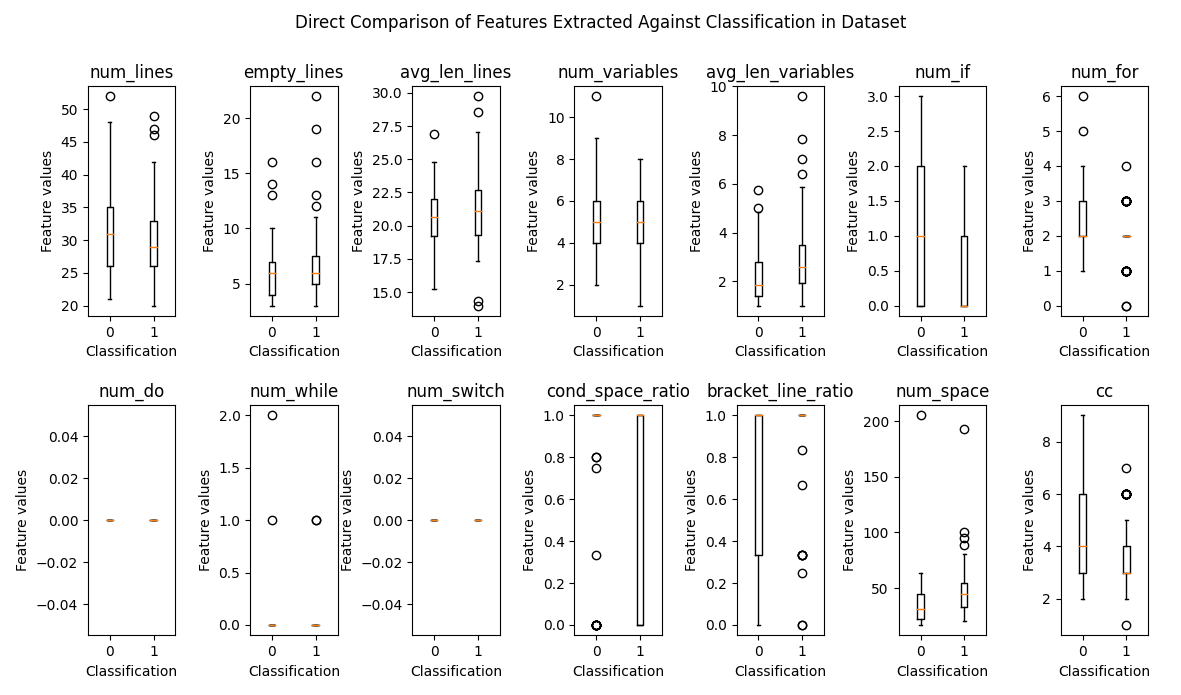
\includegraphics[width=0.8\textwidth]{figure3.3.png}
\caption{Direct comparison of features extracted against classification in the final dataset}
\end{figure}

\subsection{Features Extraction}

The list of features is extracted from the code samples with a script. Over the course of the development of the project, 2 features extractors were developed, the first one in Java and the latter one in Python. Both features extractors would read novice and expert files stored in a local folder and extract a list of features to print in the document or in memory for another component’s usage.

The original features extractor, developed in Java with the JavaParser library (JavaParser, 2021), was used in all experiments. JavaParser is a Java code parser and abstract syntax tree (AST) generator. Using JavaParser, the Java code file is broken down into tokens in the AST, allowing filtering of the types of tokens to achieve counting of the number of tokens of a type, fetching a list of token’s text of a type, et cetera. The feature extractor starts by reading all files in a folder, then checks each filename against a given list of novice or expert usernames to check if the file was created by a novice or expert for data labelling in the dataset. Then all features would be extracted from the code and the results, along with the data label would be printed in the terminal output in a CSV format. The dataset in CSV file format could then be passed to the training program.

In later stages of the project, a highly similar features extractor was developed, using Python 3 this time. This was due to a decision made to transform the entire project’s code to be in the same programming language to make its use for the website application, which is developed in Python as well, simpler. The Python version uses the javalang library (Thunes, 2021), which provides functionalities that are very close to its Java counterpart. For the Python version, instead of printing the result in CSV format in the terminal, it was made as a Python module, which would take in a filename, read its content and return the results as an array, to allow better integration with other components of the system, mainly the training part.

Below are 2 snippets of code demonstrating the extraction of a feature, number of if statements, implemented in both Java and Python feature extractors.

Java:

\begin{lstlisting}
public static void main(String[] args) {
    CompilationUnit cu = StaticJavaParser.parse(file);
    VoidVisitor<?> ifHandler = new IfHandler();
    ifHandler.visit(cu, null);
    System.out.println(((IfHandler) ifHandler).counter);
}

private static class IfHandler extends VoidVisitorAdapter<Void> {
    public int counter = 0;

    @Override
    public void visit(IfStmt n, Void arg) {
        super.visit(n, arg);
        counter++;
    }
}
\end{lstlisting}

Python:

\begin{lstlisting}
tree = javalang.parse.parse(file)
num_if = len(list(tree.filter(javalang.tree.IfStatement)))
\end{lstlisting}

\section{Training}

A list of machine learning models, listed in Table 3.2, were selected to be trained and tested for all experiments. The list consists of 10 models from a wide range of different types of models, such as linear models, neural networks and decision trees. This was done to identify the best model in experiments as well as which models generally do better with the dataset.

The model training part is done by a Python script using the scikit-learn library, a set of code developed to assist machine learning operations in Python. Taking the dataset as input, the developed code would train and evaluate the model with 10 splits k-fold cross-validation, where the script would then return the average and standard deviation of the accuracy values obtained from the training of each model.

\begin{table}[h!]
\centering
\begin{tabular}{lm{13em}l}
\hline
Initial Used & Full Name & Model Type \\
\hline
LR & Logistic Regression & Linear \\
LDA & Linear Discriminant Analysis & Discriminant Analysis \\
KNN & K-neighbours & Neighbours \\
CART & Decision Tree & Tree \\
NB & Gaussian Naive Bayes & Naive Bayes \\
SVM Lin & Support Vector Classification (with linear kernel) & Support Vector Classification \\
SVM Pol & Support Vector Classification (with polynomial kernel) & Support Vector Classification \\
SVM / SVM RBF & Support Vector Classification (with radial basis function kernel) & Support Vector Classification \\
MLP & Multi-layer Perceptron & Neural Network \\
RF & Random Forest & Ensemble \\
\hline
\end{tabular}
\caption{Models used in experiments}
\label{table:3.2}
\end{table}

\section{Results}

In this section, certain important experiments will be discussed, as well as the final model. Model accuracies are calculated as the mean of the results of the 10 split k-fold results unless elsewhere specified.

\subsection{First Experiment (Experiment 1)}

As the first-ever experiment conducted for this project, experiment 1, this experiment was conducted with the aim of setting the basis and expectations for the project. With the 12 initial features, the dataset consists of 27 rows, from 9 authors, where 5 were experts and 4 were novice developers, each contributing 3 files to the dataset. The best model in this experiment, logistic regression, achieved a 70.0\% mean-accuracy, while others achieved roughly 60\% mean-accuracy. However, it was noticed that the mean-accuracy results sounded positive for the first experiment, the range of accuracies were very wide. The standard deviation of the logistic regression model’s accuracies was 0.314, showing huge fluctuations between each run. It was concluded that the size of the dataset was too small, causing unreliable results, prompting the need for larger datasets in future experiments. The resulting model accuracy can be found in Figure 3.4.

\begin{figure}[h!]
\centering
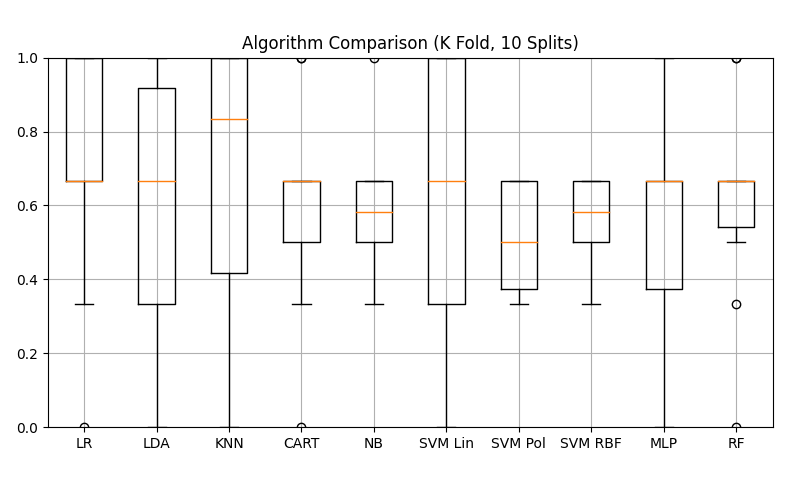
\includegraphics[width=0.8\textwidth]{figure3.4.png}
\caption{Comparison of the accuracy performance of all models in experiment 1}
\end{figure}

\subsection{Code Complexity Feature and Removal of General Code (Experiment 16 to 19)}

Experiments 16 to 19 experimented on 2 changes, the addition of the complexity feature and removal of general code from the code samples. All 4 experiments were conducted using the same set of 266 code samples, with multiple samples from 26 developers. 115 samples were from novice developers, while 151 were from experts. The differences between the 4 experiments are shown in Table 3.3 while results are included in Table 3.4.

\begin{table}[h!]
\centering
\begin{tabular}{l|ll}
\hline
& With Complexity & Without Complexity \\
\hline
With General Code & Experiment 18 & Experiment 16 \\
Without General Code & Experiment 19 & Experiment 17 \\
\hline
\end{tabular}
\caption{Differences in the settings between experiment 16 to 19}
\label{tab:3.3}
\end{table}

The complexity metric implemented in this set of experiments is a simplified version of the cyclomatic complexity, being the sum of the number of if, for, do, while and switch statements in the file. For the removal of general code, in each code samples, there is a part that is identical in each file, such as the part where it prints the function result out to standard output, these parts are provided by HackerRank in their code template. In experiment 17 and 19, these parts are removed.

\begin{table}[h!]
\centering
\begin{tabular}{l|llll|l}
\hline
& \multicolumn{4}{c|}{Experiment Number} & \\
Model & 16 & 17 & 18 & 19 & Average \\
\hline
LR & 0.674675 & 0.707792 & 0.684848 & 0.707792 & 0.693777 \\
LDA & 0.688961 & 0.683766 & 0.694156 & 0.679004 & 0.686472 \\
KNN & 0.534199 & 0.655411 & 0.566883 & 0.674242 & 0.607684 \\
CART & 0.595887 & 0.616883 & 0.586580 & 0.650866 & 0.612554 \\
NB & 0.452814 & 0.575541 & 0.457576 & 0.585065 & 0.517749 \\
SVM & 0.595455 & 0.669481 & 0.604545 & 0.669264 & 0.634686 \\
MLP & 0.693939 & 0.697835 & 0.684199 & 0.697619 & 0.693398 \\
RF & 0.638095 & 0.707792 & 0.638312 & 0.688961 & 0.668290 \\
\hline
Average & 0.609253 & 0.664313 & 0.614637 & 0.669102 & \\
\hline
\end{tabular}
\caption{Average model accuracies recorded in experiment 16 to 19}
\label{tab:3.4}
\end{table}

Comparing the 4 best models in experiment 18 to 16 and 19 to 17, it could be concluded that the complexity feature did not add value to the model. In experiments 18 and 16, both with general code, the addition of the complexity feature increased the accuracy by 0.22\%. While in experiments 19 and 17, both without general code, the feature’s addition decreased the accuracy by 0.85%.

Similarly, by comparing the 4 best models in experiment 16 to 17 and 18 to 19, conclusions regarding the effect of removing general code could be drawn. In experiments 16 and 17 both without complexity, the removal of general code improved the accuracy by 3.77\%. While in experiments 18 and 19, the same measure also improved the accuracy by 2.66\%. This shows that removing general code deals a positive impact on the model’s performance.

\subsection{Halstead Metrics (Experiment 20 to 23)}

In this set of experiments, the target was to evaluate the effect of the addition of the 6 Halstead metrics on the model’s accuracy. This set of experiments are identical to that of experiments 16 to 19, except that for each dataset the 6 new features were added. Table 3.5 shows the full results from all 4 experiments, while Table 3.6 compares the accuracy of the best 4 models in experiments 16 to 19 with experiments 20 to 23.

As discussed in the background section, Halstead metrics is a set of metrics set by Halstead (1977) to evaluate a piece of code. The set of metrics, same as that implemented by this set of experiments, includes program vocabulary, program length, calculated estimated program length, volume, difficulty and effort.

\begin{table}[h!]
\centering
\begin{tabular}{l|llll|l}
\hline
& \multicolumn{4}{c|}{Experiment Number} & \\
Model & 20 & 21 & 22 & 23 & Average \\
\hline
LR & 0.660823 & 0.688528 & 0.665584 & 0.683983 & 0.674730 \\
LDA & 0.683983 & 0.664719 & 0.674892 & 0.669481 & 0.673269 \\
KNN & 0.580519 & 0.534199 & 0.580519 & 0.534199 & 0.557359 \\
CART & 0.670130 & 0.612554 & 0.660173 & 0.598268 & 0.635281 \\
NB & 0.655195 & 0.590693 & 0.659957 & 0.600000 & 0.626461 \\
SVM & 0.585065 & 0.566234 & 0.585065 & 0.570779 & 0.576786 \\
MLP & 0.636797 & 0.627056 & 0.552381 & 0.565584 & 0.595455 \\
RF & 0.680519 & 0.679654 & 0.670996 & 0.665584 & 0.674188 \\
\hline
Average & 0.644129 & 0.620455 & 0.631196 & 0.610985 \\
\hline
\end{tabular}
\caption{Average model accuracy values recorded in experiment 20 to 23}
\label{tab:3.5}
\end{table}

\begin{table}[h!]
\centering
\begin{tabular}{l|ll|l}
\hline
Model & 16-19 Average & 20-23 Average & Difference \\
\hline
LR & 0.693777 & 0.674730 & -2.75\% \\
LDA & 0.686472 & 0.673269 & -1.92\% \\
MLP & 0.693398 & 0.595455 & -14.13\% \\
RF & 0.668290 & 0.674188 & 0.88\% \\
\hline
Average &  &  & -4.48\% \\
\hline
\end{tabular}
\caption{Comparison of the difference in model accuracy between experiment 16 to 19 and 20 to 23}
\label{tab:3.6}
\end{table}

As seen in Table 3.6, in the best 4 models from both sets of experiments, adding Halstead metrics as a feature led to a 4.48\% decrease in the accuracy on average. 3 of the models were made less accurate by the new set of features, while the model that benefited from the addition only gained a 0.88\% improvement in accuracy. Therefore the conclusion was drawn that Halstead metrics should not be included in the final list of features.

\subsection{JHawk Metrics (Experiment 24 to 25)}

This set of experiments were designed to evaluate if the addition of the 32 JHawk metrics would help improve the accuracy of the models. Due to the complexity in extracting JHawk metrics from the code samples, only 157 rows of data were collected, all originally from experiment 19 (with the complexity feature but general code removed). Firstly, to establish a baseline, the same 157 selected entries from experiment 19 were given to the models. For experiment 24, JHawk metrics were extracted from the 157 code samples and directly used as the dataset. For experiment 25, the extracted JHawk metrics were combined with the original set of features used in experiment 19. The results of each experiment and a basic comparison are shown in Table 3.7.

JHawk is a software designed to evaluate Java programs (Virtual Machinery, 2021). The software uses a wide range of metrics to do so. In this set of experiments, code samples were fed to JHawk and the following list of 32 features were extracted using the tool: number of methods, average cyclomatic complexity, Halstead bugs cumulative value, unweighted class size, CBO, number of comment lines, review factor value, depth of inheritance tree, specialization ratio, cohesion, maximum cyclomatic complexity, number of query methods, number of superclasses, number of subclasses, number of command methods, Halstead length cumulative value, lack of cohesion of methods, number of Java statements, Halstead effort cumulative value, total response for class, maintainability index, number of lines of code, fan in, ReUse ratio, LCOM2, Halstead volume cumulative value, fan out, SIX, total cyclomatic complexity, MPC, number of comments.

\begin{table}[h!]
\centering
\begin{tabular}{l|lll|ll}
\hline
& \multicolumn{3}{c|}{Experiment} & & \\
Model & 19 (159 rows) & 24 JHawk Only & 25 Combined & 19 vs. 24 & 19 vs. 25 \\
\hline
LR & 0.673750 & 0.485256 & 0.662821 & -27.98\% & -1.62\% \\
LDA & 0.685833 & 0.436538 & 0.564744 & -36.35\% & -17.66\% \\
KNN & 0.595000 & 0.492949 & 0.492949 & -17.15\% & -17.15\% \\
CART & 0.565833 & 0.580769 & 0.560897 & 2.64\% & -0.87\% \\
NB & 0.487500 & 0.469231 & 0.509615 & -3.75\% & 4.54\% \\
SVM & 0.679583 & 0.540385 & 0.540385 & -20.48\% & -20.48\% \\
MLP & 0.628750 & 0.540385 & 0.540385 & -14.05\% & -14.05\% \\
RF & 0.597083 & 0.555128 & 0.596795 & -7.03\% & -0.05\% \\
\hline
Average &  &  &  & -15.52\% & -8.42\% \\
\hline
\end{tabular}
\caption{Average model accuracy values recorded in experiment 24 to 25 with basic comparison statistics}
\label{tab:3.7}
\end{table}

As seen in Table 3.7, in almost all cases, JHawk metrics, no matter if alone or combined with existing features, underperforms the existing set of features quite significantly, with an average of 15.5\% and 8.42\% decrease in accuracy when comparing the original set of features with JHawk metrics only and combined respectively. The results suggest that JHawk metrics should not be included in the final set of features.

\subsection{Final Model (Experiment 40)}

Experiment 40 was the experiment conducted under this project that set the final model to be used in the entire project. The dataset consisted of 164 rows, from 164 different authors all solving the same coding question, where 91 of them were experts and 73 were novice developers. This experiment used the final list of features as shown in Table 3.1. A comparison of all model’s accuracy is shown in Figure 3.5. The coefficients found in the best performing model, logistic regression which achieved a 69.0\% accuracy and 0.0936 standard deviation across the results from all 10 splits, for each feature is shown in Figure 3.6.

\begin{figure}[h!]
\centering
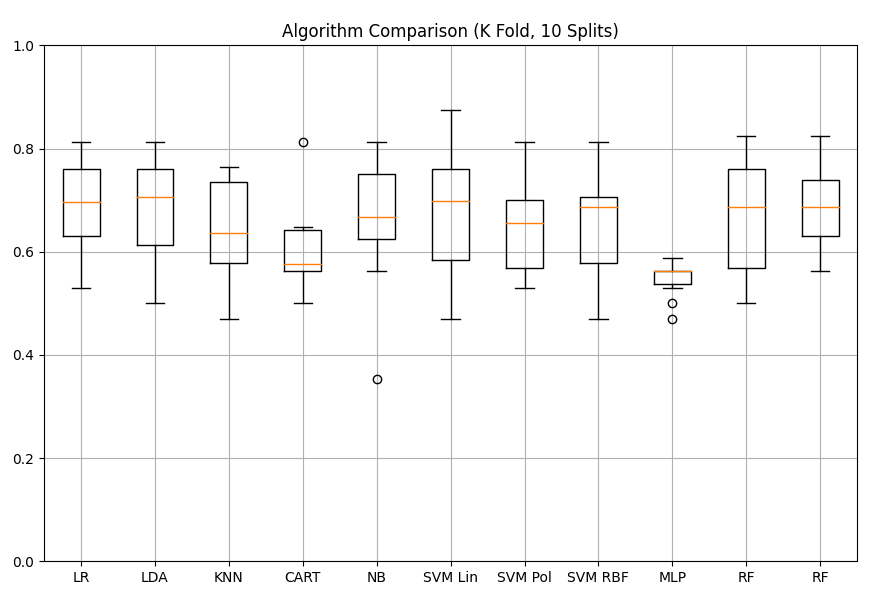
\includegraphics[width=0.8\textwidth]{figure3.5.png}
\caption{Comparison of model accuracy values in experiment 40}
\end{figure}

\begin{figure}[h!]
\centering
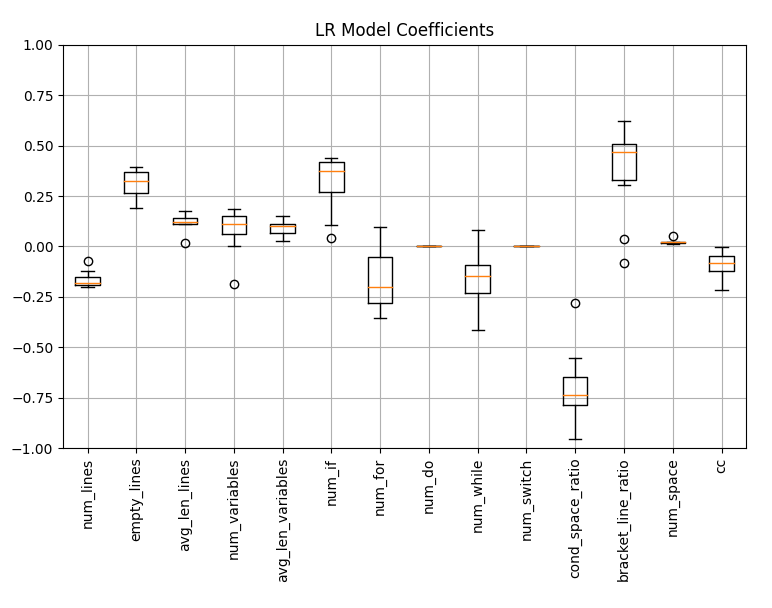
\includegraphics[width=0.8\textwidth]{figure3.6.png}
\caption{Coefficients found in the final logistic regression model}
\end{figure}

\subsection{Features Normalization (Experiment 41 and 42)}

An additional set of experiments were performed to evaluate the impact of data scaling on the accuracy of the models. 2 additional experiments were made, using the same set of data from experiment 40. In experiment 41, a min-max scaler had been applied to the dataset, mapping all values in each feature to a minimum of 0 and a maximum of 1. In experiment 42, a standard scaler had been applied to the dataset, mapping all values in each feature to a new range, setting the standard deviation of all values to 1. The results, with comparison data, can be found in Table 3.8, with the name of the best 4 models in experiment 40 highlighted. The conclusion of this set of experiments was that data normalization does not help improve the accuracy of the models.

\begin{table}[h!]
\centering
\begin{tabular}{l|lll|ll}
\hline
& \multicolumn{3}{c|}{Experiment} & & \\
Model & 40 & \makecell{41 \\ (Min-Max Scaling)} & \makecell{42 \\ (Standard Scaling)} & 40 vs. 41 & 40 vs. 42 \\
\hline
\textbf{LR} & 0.689706 & 0.683088 & 0.683456 & -0.96\% & -0.91\% \\
\textbf{LDA} & 0.688971 & 0.688971 & 0.688971 & 0.00\% & 0.00\% \\
KNN & 0.635294 & 0.603676 & 0.561765 & -4.98\% & -11.57\% \\
CART & 0.603676 & 0.597426 & 0.597426 & -1.04\% & -1.04\% \\
NB & 0.659559 & 0.659559 & 0.659559 & 0.00\% & 0.00\% \\
\textbf{SVM Lin} & 0.684191 & 0.598162 & 0.672059 & -12.57\% & -1.77\% \\
SVM Pol & 0.647794 & 0.641176 & 0.615441 & -1.02\% & -4.99\% \\
SVM RBF & 0.646324 & 0.665441 & 0.616544 & 2.96\% & -4.61\% \\
MLP & 0.548897 & 0.573162 & 0.615074 & 4.42\% & 12.06\% \\
\textbf{RF} & 0.670588 & 0.670588 & 0.670588 & 0.00\% & 0.00\% \\
\hline
Average & & & & -1.32\% & -1.28\% \\
\hline
\end{tabular}
\caption{Results from experiment 40 to 42, with the best 4 models in experiment 40 highlighted, and results between each experiment compared}
\label{tab:3.8}
\end{table}

\subsection{Conclusion of the Experiments}

Above mentioned, are all key experiments conducted that had a significant impact on decisions made on the training of the final model. As a result of all these experiments, it was decided that the logistic regression model in experiment 40 shall be used as the final model. With 164 pieces of code, each from a different author solving the same coding question, extracting the 14 features as listed in Section 3.2.1, without data normalization, the final model has a 69.0\% accuracy when evaluated under 10 split k-fold cross-validation.

\chapter{Prototype Application}

One of the prototypes developed was a website application, targeting individual users who would like to evaluate their code or just try the model out. The design, implementation and evaluation of the prototype developed will be discussed in the following sections.

\section{Design}

\subsection{Requirements}

For the website application, a list of requirements, both functional and non-functional, were drawn up to assess the final product and guide development.

For functional requirements, the system shall:

\begin{itemize}
\item Show the user a coding question
\item Take the user’s code as input
\item Evaluate the code input using the model
\item Show the results from the model
\item Have instructions on how to proceed on different parts of the website
\end{itemize}

For non-functional requirements, the system should:

\begin{itemize}
\item Be designed to be visually appealing
\item Have clear instructions on-screen that users can easily understand
\item Be easy to navigate to different parts of the website
\item Include a simple description of the project
\end{itemize}

\subsection{System Architecture}

As a simple website application, the user would interact with the front end component of the system to submit their code and get the result from the model. The server can be split into 3 main components: front end, features extractor and model. The front end component would pass the code submitted to the features extractor after making basic validations to the submission. The features extractor would then parse the code and output an array of the values corresponding to each feature extracted. The array is then passed into the model to get the classification. Finally, the classification is delivered to the user.

\begin{figure}[h!]
\centering
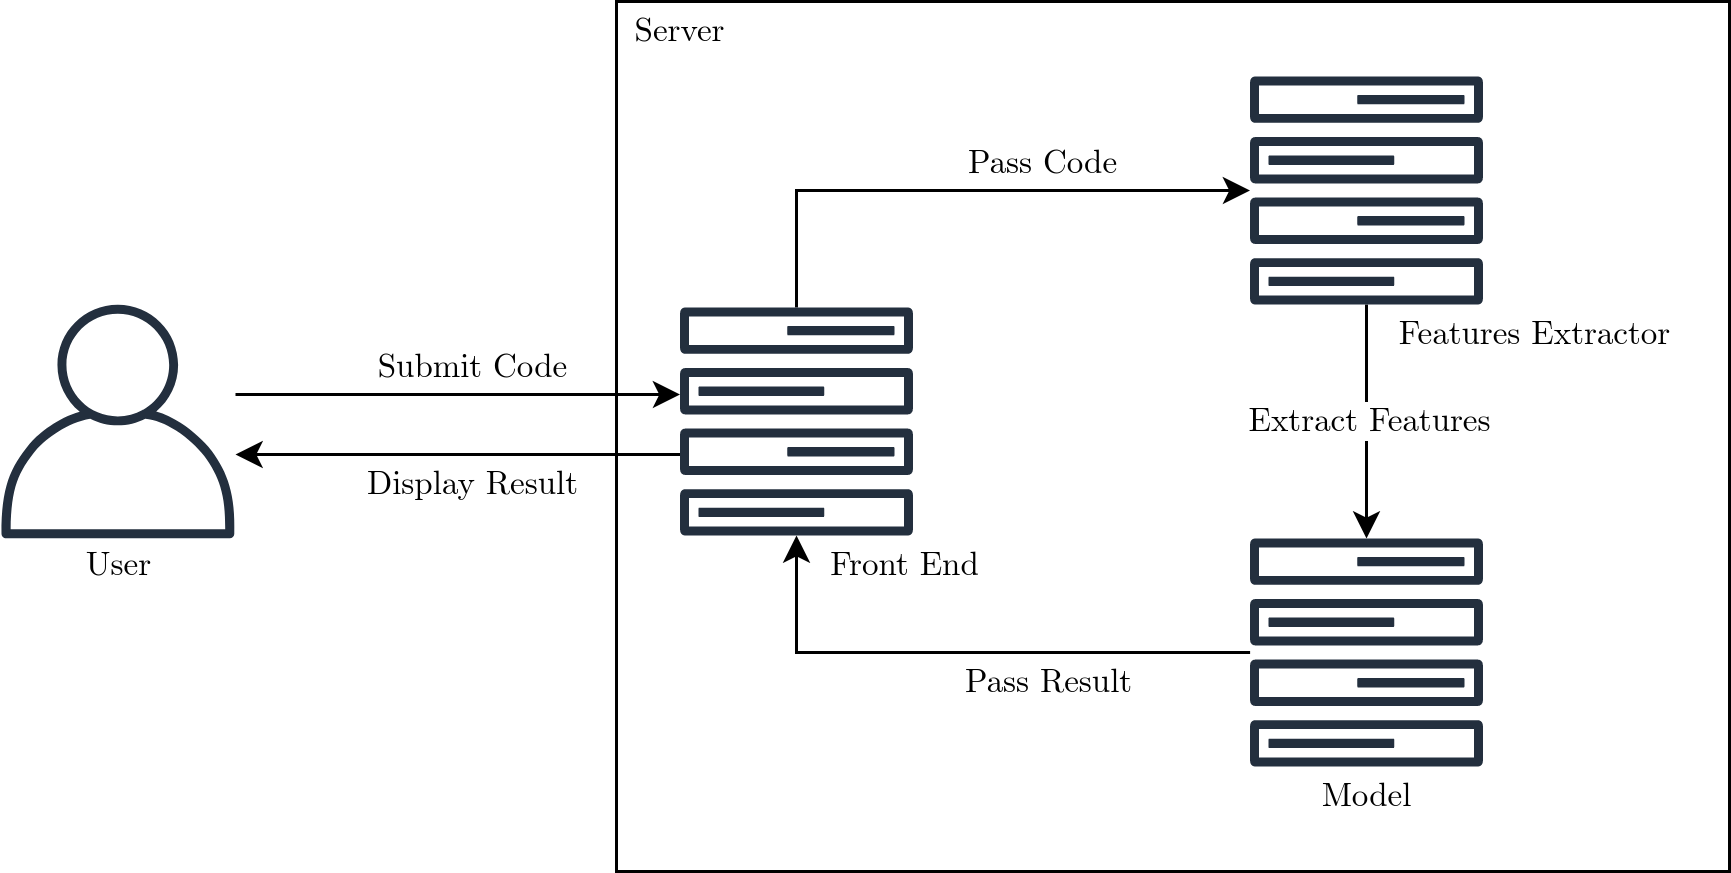
\includegraphics[width=0.8\textwidth]{figure4.1.png}
\caption{The designed components in the system}
\end{figure}

\subsection{Use Cases}

There is one main use case for the website application, details of the use case is presented in Table 4.1.

\begin{table}[h!]
\centering
\begin{tabular}{|m{7em}|m{28em}|}
\hline
\multicolumn{2}{|l|}{Use case: Obtain a developer’s experience classification} \\
\hline
Description & An actor uses the website application to evaluate one’s development experience \\
\hline
Actors & Individual users who would like to use the developed model to assess the actor’s own or other’s development experience \\
\hline
Pre-conditions & (none) \\
\hline
Assumptions & The actor is able to perform basic Java programming \\
\hline
Main flow & 
\begin{enumerate}
\item The actor lands at the homepage
\item The actor navigates to the application page
\item The actor downloads the 2 supplied files and completes Solution.java
\item The actor uploads the completed Solution.java
\item The actor submits the form
\item The system extracts features from the uploaded file
\item The system passes those features to the model
\item The system shows the user the classification obtained from the model
\end{enumerate} \\
\hline
Post-conditions & The actor is presented with the classification \\
\hline
Extensions & Step 6) If the file contains a syntax error, the system shows an error and go back to step 4 \\
\hline
\end{tabular}
\caption{Use case table for obtaining a developer’s experience classification}
\label{tab:4.1}
\end{table}

\subsection{User Interface Concept}

Prior to working on the implementation, a simple wireframe prototype for the key parts of the website was created using Figma, a prototyping tool, allowing some interactions with the wireframe pages. This process provides a preview of how the pages would look and function, to prevent any obvious design mistakes from only being realized at a later stage.

At this stage, there were 2 main pages, including the homepage, which accepts the user’s code, and the results page, which shows the classification result from the model. The wireframe for the 2 pages could be seen in Figures 4.2 and 4.3.

\begin{figure}[h!]
\centering
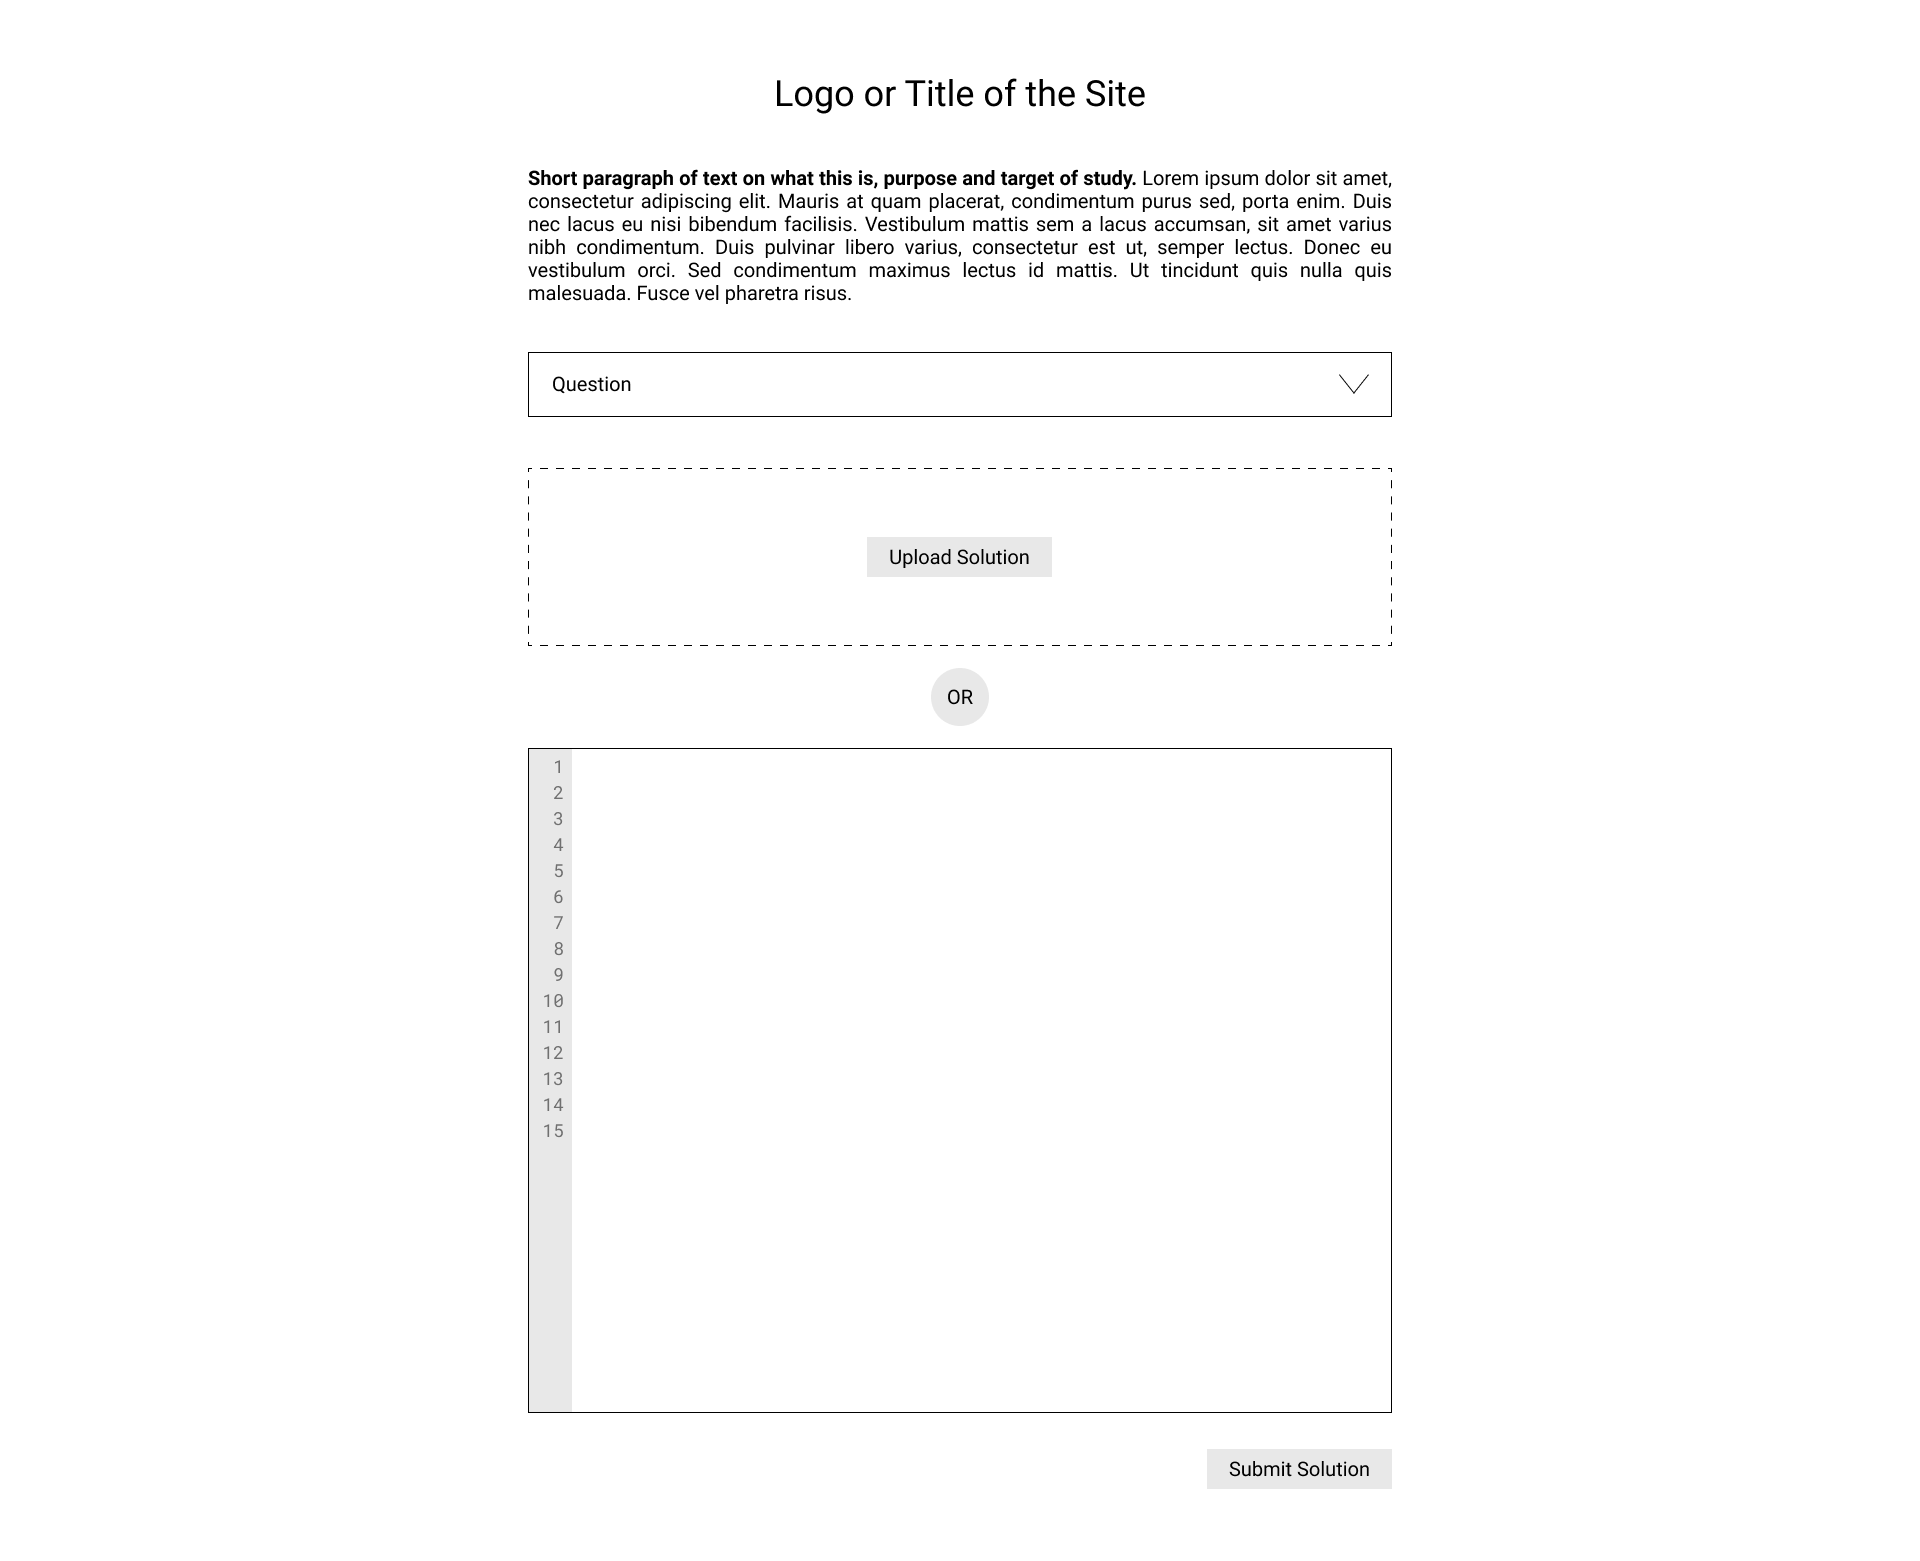
\includegraphics[width=0.8\textwidth]{figure4.2.png}
\caption{Mockup of the homepage of the website}
\end{figure}

\begin{figure}[h!]
\centering
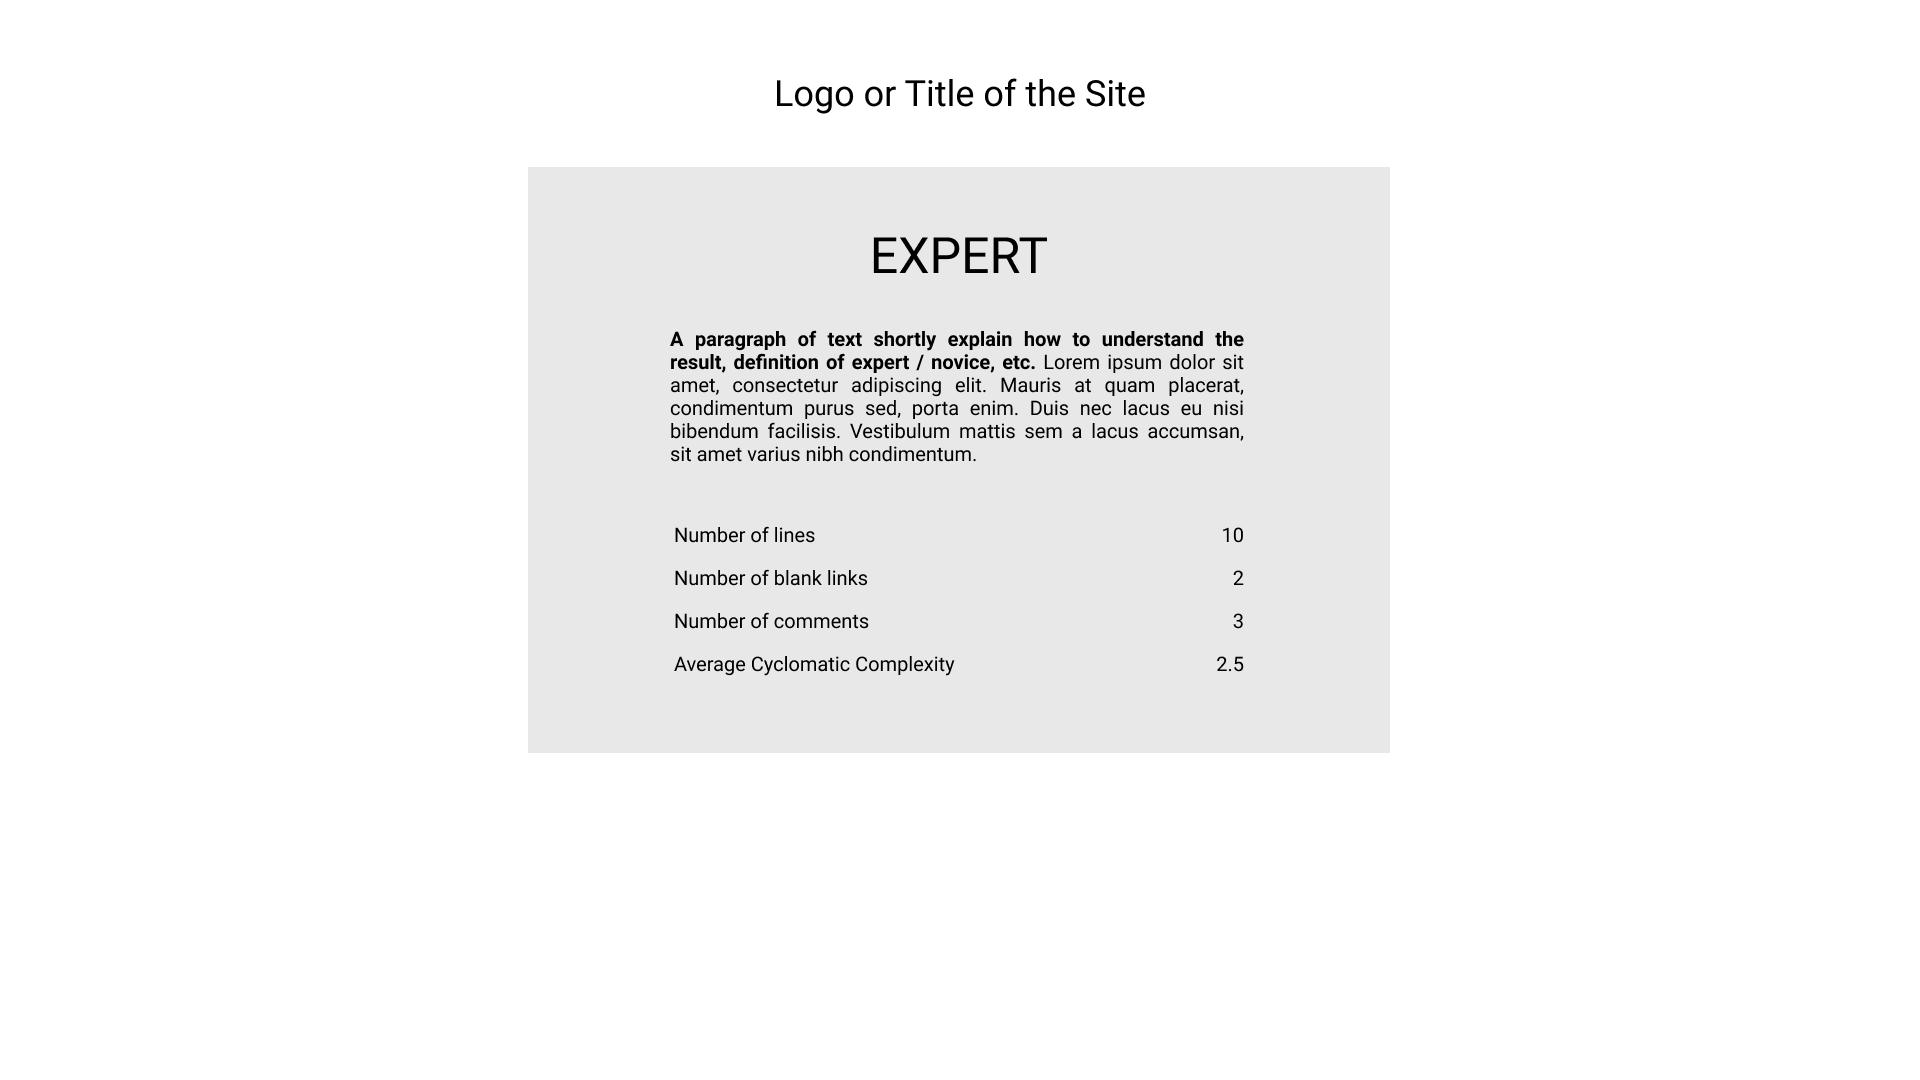
\includegraphics[width=0.8\textwidth]{figure4.3.png}
\caption{Mockup of the results page of the website}
\end{figure}

It was considered whether the site should record the user’s input and, automatically or manually, feed feedback back to the model to further improve it. It was concluded that this should not be done for a number of reasons. Firstly, the model is very fragile, with only 164 rows in the final dataset and a 69.0\% accuracy, the model is not mature enough to accept additional data from a similar but different data source, which could have a negative effect on the model. Besides, the site was not designed for this purpose, users were not told extremely clear how novice and expert developers were classified, especially in special and edge cases. Including mislabeled data in a small dataset could easily damage the model. Finally, the website was designed as a prototype, to demonstrate possible uses of the model developed and to experiment with the use of machine learning models in a website for personal uses, a feedback mechanism did not seem very beneficial and crucial to the system. Therefore, it was concluded that it was not appropriate, in this situation, to implement the automatic training feedback feature.

\section{Implementation}

\subsection{Development Environment}

For this website application, Python was selected as the programming language to be used on the server. This is mainly due to the model being developed using Python code as well. By using Python in both the model and server, it is possible to simply export the trained model as a serialized object to the file and import the exact same object onto the server. While it is possible to extract all details of a model, the chosen approach is much simpler and time-efficient.

Atom was used as the code editor, with plugins to support Python code linting according to the PEP8 and Flake8 standards. The code was developed to abide by most of those style guidelines.

The server is developed using Flask, a simple but popular python web server framework. It was chosen over other similar frameworks such as Django based on the amount of personal experience with the framework. The framework handles all browsing sessions, incoming requests, error responses et cetera. Below is a snippet of code, serving a webpage, highlighting the simplicity of using Flask.

\begin{lstlisting}
from flask import Flask, render_template, session

app = Flask(__name__)
app.config['SECRET_KEY'] = '<app secret key>'.encode('utf8')

@app.route('/')
def home():
    return render_template('home.html',
                           mode=session.get('mode'))

\end{lstlisting}

The render\_template function, widely used in this application, is provided by Flask, and renders a web page using the Jinja template engine. Following is a snippet of code showing the usage of the Jinja template syntax to render a link to a web page on the site.

\begin{lstlisting}
<a href="{{ url_for('app_route') }}">[Try It Out]</a>
\end{lstlisting}

\subsection{Homepage}

During implementation, it was realized that it is better to separate introductory text from the main application part itself to create a better feel of coherence throughout the site. Therefore a separate application page was developed to hold the coding question and to take user input. While the homepage introduces the website.

The functional aim for the homepage is to introduce the website, what it is and how it works. At the top of the page, it shows the name of the site, Coding Expert Detector, and a one-sentence statement, marked “TL;DR”, for those who do not prefer reading a lot and would just want to know what the website is about as quickly as possible.

It is then followed by a simple 3 step description, with an illustration diagram, of how the model is trained and used on the site. The diagram, which provides a simple visual explanation of the above, is created in the SVG format using Inkscape, an open-source vector graphic design software,  to allow unlimited resizing.

Finally, the page introduces the creator, this project and its supervisor.

\begin{figure}[h!]
\centering
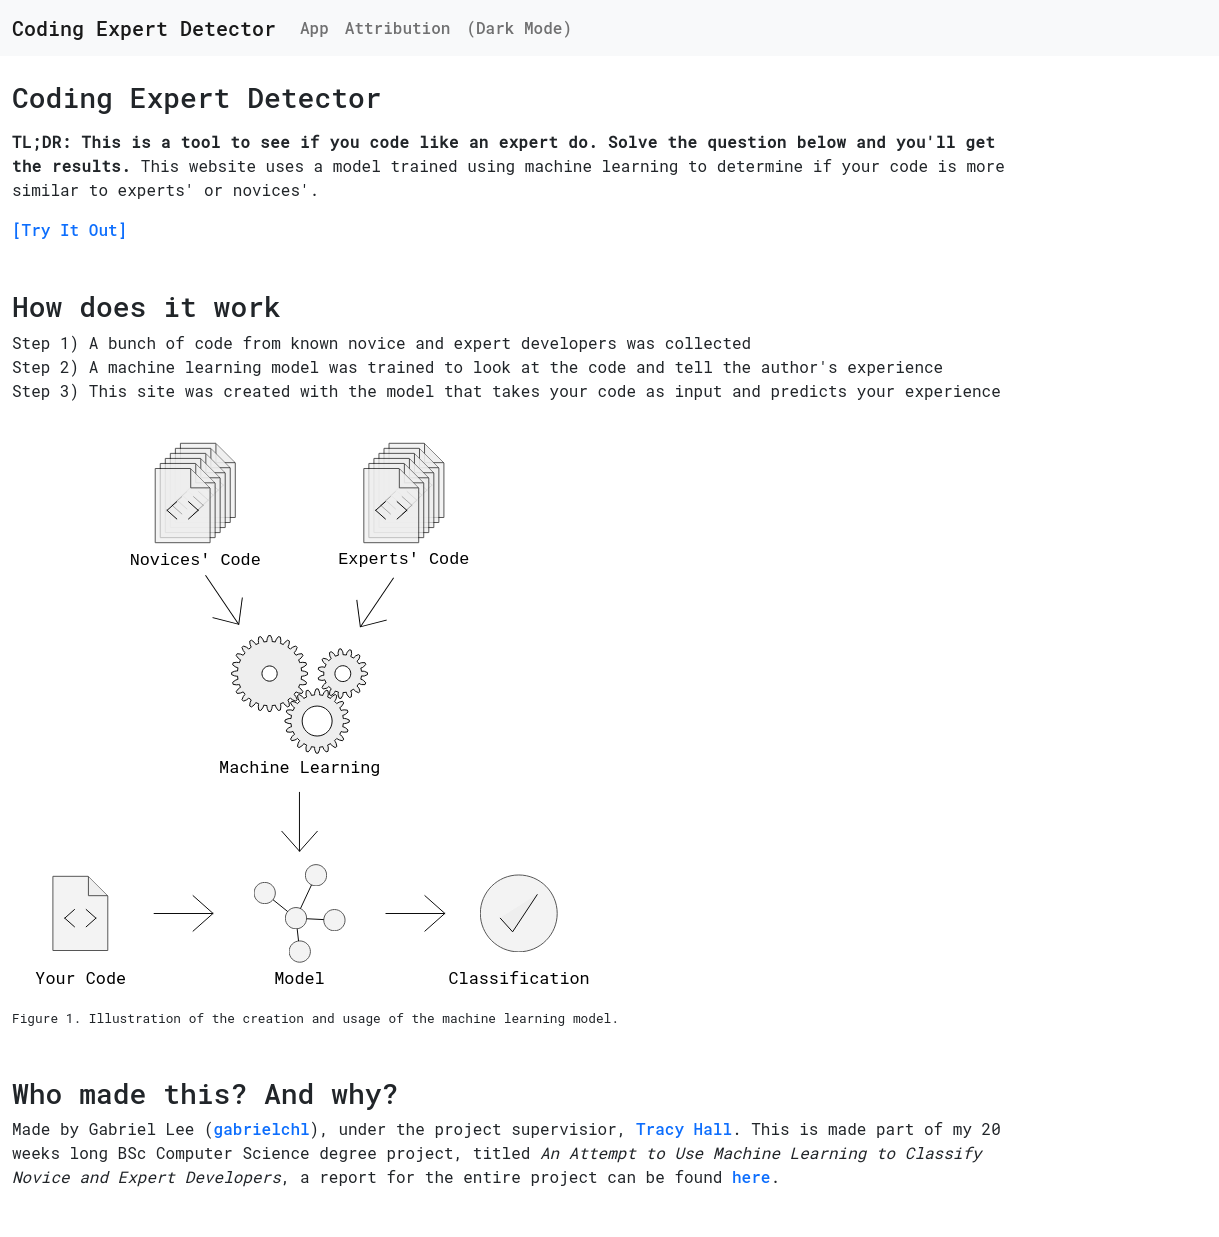
\includegraphics[width=0.8\textwidth]{figure4.4.png}
\caption{Screenshot of the homepage}
\end{figure}

\subsection{Application Page}

For the application page, there are only 2 functional aims, display the coding question and take the user’s solution code as input. As the page contains quite a lot of content and text, it was split into 4 main steps to assist the user in determining what they were supposed to do at the next step.

The first step was to “read the following question”. The question is displayed on the screen, with all mathematical symbols rendered using MathJax, a Javascript library for rendering mathematical scripts elegantly.

The second step was to “download the following files and complete the task”. 2 files were provided, Solution.java and Test.java. Solution.java provides the code template for the user to start working on. This template is highly similar to that used in the training dataset to ensure that there are no systematic changes to the data input, causing the model to not be able to identify some features. For Test.java, it provides some test cases for the user to run against their code to confirm that their code works before submitting. The text on the application page instructs the user to not modify certain parts of the template, as well as suggests how to run those test cases. Figure 4.5 shows the output of the test file with several failed test cases.

\begin{figure}[h!]
\centering
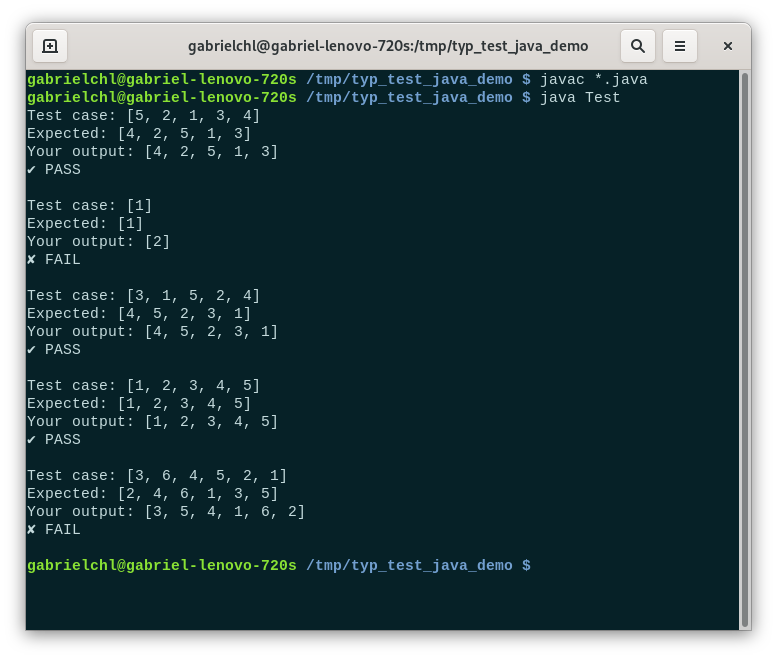
\includegraphics[width=0.8\textwidth]{figure4.5.png}
\caption{Screenshot of an example output of the test file featuring 2 failed test cases}
\end{figure}

The third step was to “upload your solution”. The user would upload their Solution.java using a regular file selector button. The code read from the file is then displayed below the file selector button for the user to confirm the file selection. The code viewer is implemented using CodeMirror, an open-source javascript library.

Finally, step 4 includes a very visible submit button, which concludes this page.

\begin{figure}[h!]
\centering
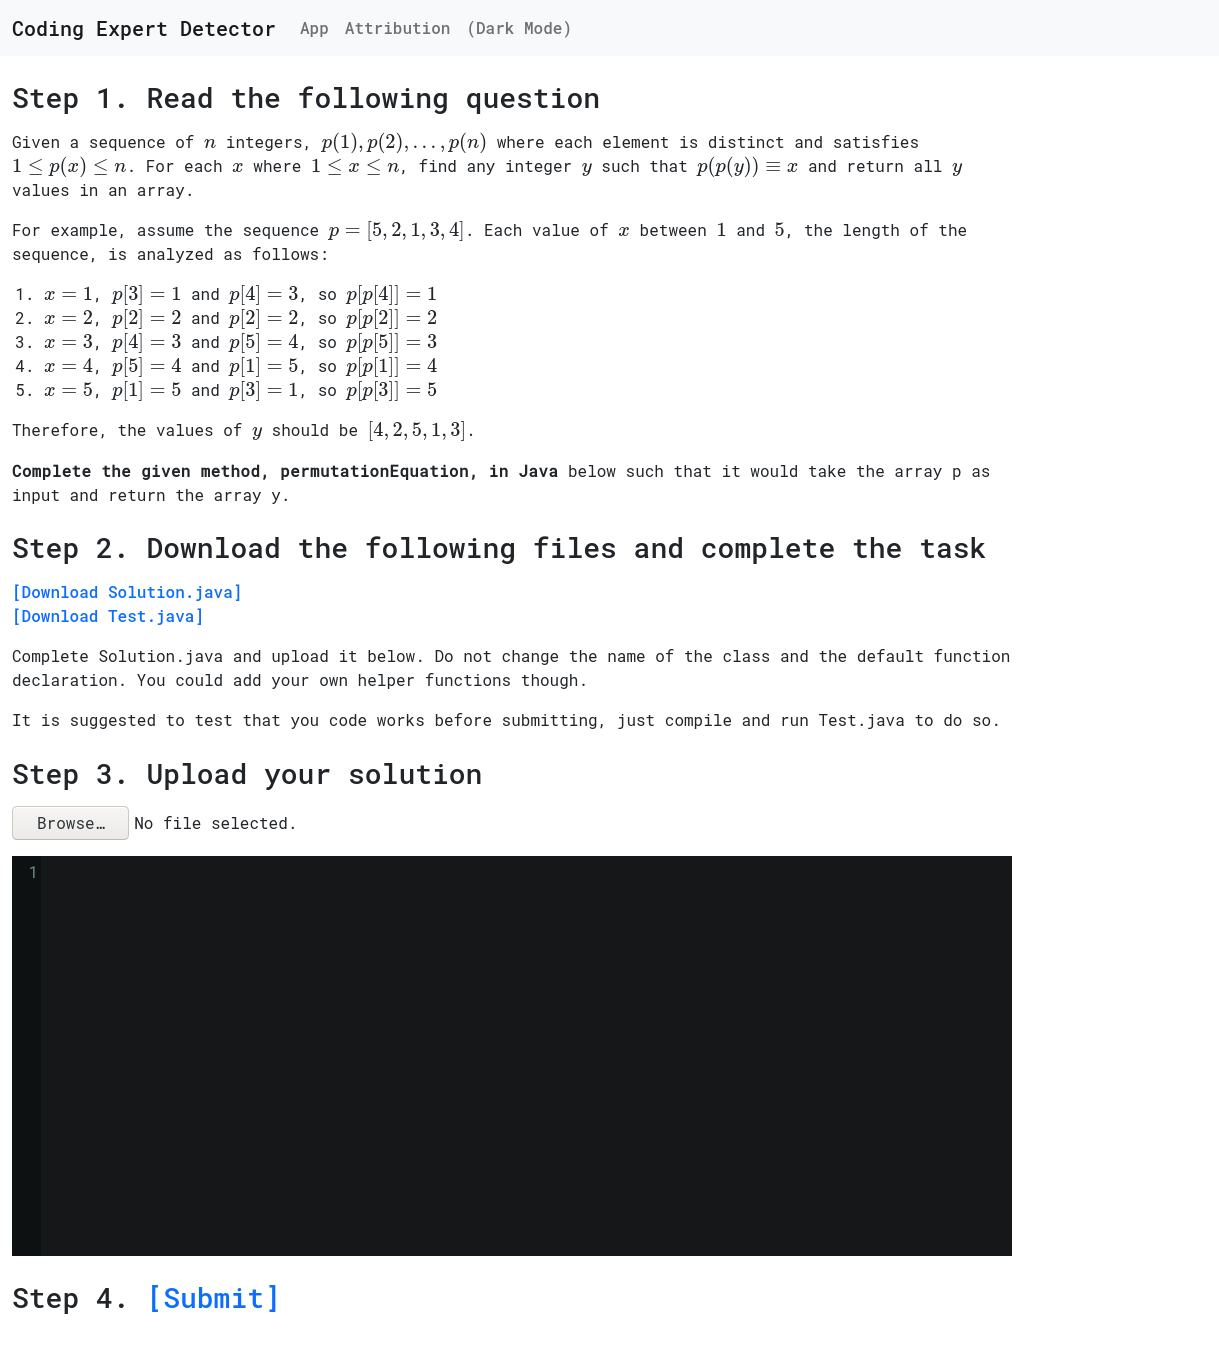
\includegraphics[width=0.8\textwidth]{figure4.6.png}
\caption{Screenshot of the application page}
\end{figure}

\subsection{Results Page}

For the results page, it simply shows the classification calculated by the model with the values of the features extracted. As the classification is the main content to show, it enjoys a significantly large font-size. The values of the features extracted is displayed in a table with the cursor hover highlighting feature. The model is loaded from a file containing the model as a serialized Python object, as shown in the following code snippet.

\begin{lstlisting}
model = joblib.load('model.sav')
prediction = model.predict([features])[0]
\end{lstlisting}

\begin{figure}[h!]
\centering
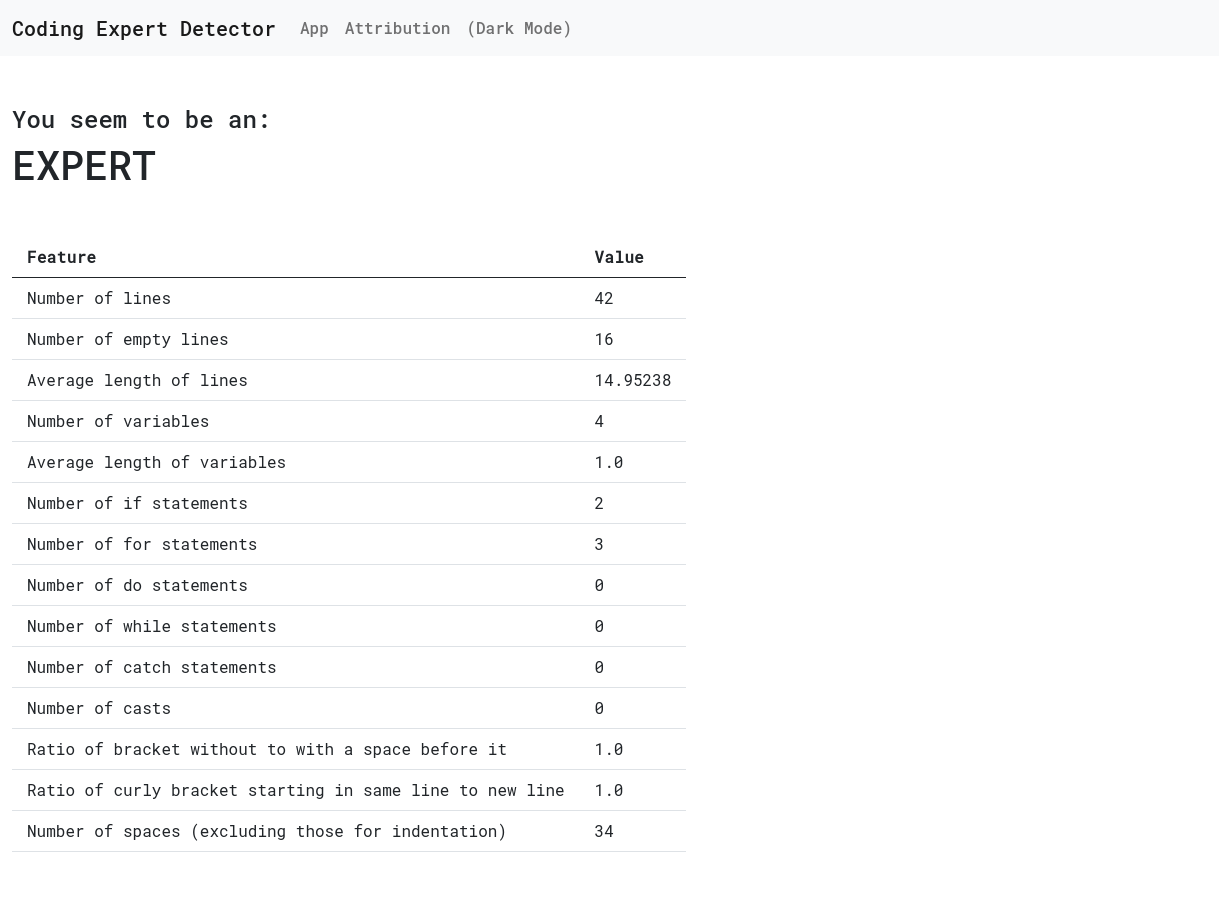
\includegraphics[width=0.8\textwidth]{figure4.7.png}
\caption{Screenshot of the results page}
\end{figure}

\subsection{Special Features}

Besides the above-mentioned pages, there is 1 feature and another page that is worth mentioning.

The main user group who would use this site is people who would like to know how experienced in programming they are when compared to others or those who would just like to try out the website and see what classification it gives. These people, mostly individual developers, would prefer if the mainly white-coloured user interface has a dark mode feature, similar to that provided in all mainstream code editors. Therefore a dark mode feature is created for the site. The trigger is on the navigation bar of the website, where the user’s preference would be stored on the web server along with the user’s browsing session so that the colour preference is kept throughout the session.

A page that was not mentioned above is the attribution page, which contains attribution text for this website, and this website only. For this website, the attribution page contains one entry regarding where the idea of the design of the visual elements of the website came from. This will be further discussed in the following section.

\begin{figure}[h!]
\centering
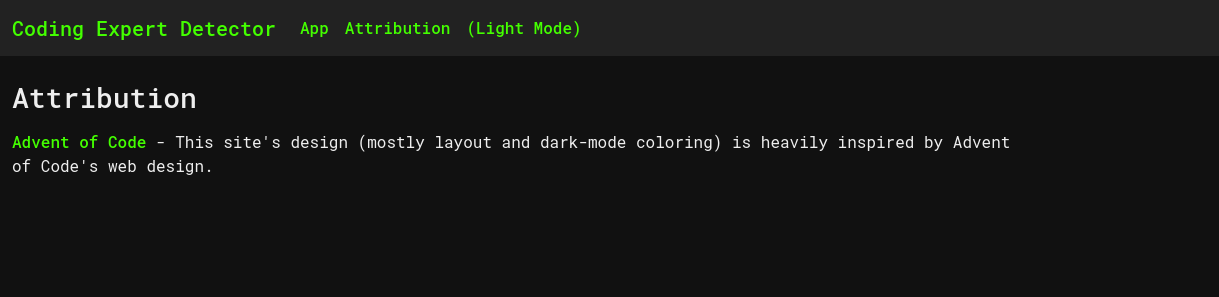
\includegraphics[width=0.8\textwidth]{figure4.8.png}
\caption{Screenshot of the attribution page in dark mode}
\end{figure}

\subsection{Design}

Bootstrap, a CSS framework by Twitter, was used for the design of the website. Bootstrap provides a range of basic elements for web developers to quickly build a website. Some elements used include links, navigation bars, tables, et cetera. Using this framework, the basic structure was created.

While Bootstrap does provide a very simple design, its elements’ size and colour make the website look just like another generic site. Therefore the design needed to be customized. Using custom CSS rules, in addition to what Bootstrap provides, the colouring for both light and dark mode, text position and font was modified, as well as some other minor changes. Parts of the design, including the font and layout, was inspired by the website of Advent of Code, an annual coding competition held in December. Such information was included on the attribution page.

\section{Evaluation and Testing}

\subsection{Semi-structured Interviews}

To evaluate different aspects, including functionality and design, of the website, 2 semi-structured interviews were conducted, one with a novice developer and the other with an expert. The aim of the 2 interviews was to collect user feedback on the website, especially when users tend to be able to give feedback on issues developers themselves could not find or are not aware of. They were introduced to the project and the developed website and asked to use the site, with a minimal amount of instructions given by the interview instructor. A list of questions was prepared prior to the interviews:

\begin{enumerate}
\item Can you tell me about your experience with coding, and Java?
\item Can you tell me about your educational credentials? What did you study and when did or will you graduate?
\item Do you think that the instructions were clear?
\item How easy is it to navigate around the site?
\item What do you think about the design of the site? Colouring, font, layout, et cetera.
\item What do you think about the presentation of the question, on a scale from 1 to 10, how hard is it to understand?
\item What do you think about the question itself, on a scale from 1 to 10, how hard is it to solve?
\item What do you think about the results? Do you agree with the classification?
\item Are there any things you would like to add?
\end{enumerate}

Besides the above questions, some followup questions and questions inspired by observing their use of the site were also asked. An example of these questions is “I saw that you spent quite a long time between reading the question and starting with your solution, what were you thinking or doing at the time?”. The length of the interviews was around 1 hour for interviewee 1, and 20 minutes for interviewee 2, with both successfully using the site and giving very high-quality feedback. Below is a short introduction to the background of both interviewees.

Interviewee 1 is a male United Kingdom university student, currently enrolled in a Computer Science Bachelor degree, completing his year 3 studies. He does not have any work experience nor commercial software development experience. Interviewee 1 has basic knowledge in the Java programming language, mostly gained in the prior 2 years from the university’s lectures.

Interviewee 2 is a male United States university student, currently enrolled in a Computer Engineer Bachelor degree, completing his year 4 studies. He is experienced in software development. Completing his software engineer internship at Google in summer 2020 working on Linux kernel development, he is set to work at Google as a software engineer after graduation in 2021.

Below is a list of feedbacks collected during the interviews:

\begin{itemize}
\item Both enjoyed the dark mode toggle ability.
\item Both found the question hard to understand. Interviewee 1 spent at least 3.7 minutes reading and understanding the coding task, requiring the interviewer’s intervention to explain the question. Interviewee 2 said that “Just say that it is a shuffled array, this is such a complex expression”.
\item Both agreed that it is easy to navigate around the site. Interviewee 2 suggested adding an additional link to the app at the bottom of the home page.
\item Interviewee 1 suggested that the text used to introduce the project on the homepage could be further simplified.
\item Interviewee 1 found it slightly hard to solve the question, giving a 6 out of 10, where 10 is that it is very hard to solve.
\item Interviewee 2 did not realize that the array provided in the question has its index starting from 1 until 3 minutes into solving the question. The interviewee hated this fact and said that “Please stop using 1-based arrays” and “I have to convert it to 0-base then to 1-base, it’s just 2 extra steps”.
\item Interviewee 2 suggested that the website should provide direct on-site testing, instead of having the user download the test file and run it locally.
\item Both agreed that while they’re satisfied with the results page design, it would be ideal to include additional information such as what features are more associated with each classification.
\end{itemize}

\subsection{Changes Proposed in the Interviews}

In this section, changes proposed by the interviewees or inspired by the 2 interviews will be discussed. Changes implemented post-interviews will be covered. As well as the discussion on certain changes to not be implemented.

The most important change that was suggested by both interviewee was that the question was hard to understand. The following changes were made to simplify parts of the question by introducing the problem from a spoken approach rather than a mathematical approach, while not giving any additional hints to solving the question to keep the input true to the training dataset. The first sentence was modified from “Given a sequence of n integers, p(1), p(2),..., p(n) where each element is distinct and satisfies 1 <= x <= n.” to “p is a shuffled array of n integers, where all integers from 1 to n are in the array.”. Additionally, the statement “Note that the array $p$ is 1-based.” was also added to the end of the question.

A minor change made to the website was to add an additional “try it out” button at the bottom of the home page, as suggested by interviewee 2, that helps people who read the entire homepage easily reach the app page from the bottom of the homepage.

Finally, as both interviewees have agreed, more information was added to the results page. To show more data to help the user interpret the values of the features extracted, a box plot is added next to all values in the results page, showing where their code stands in the dataset, shown in Figure 4.9. Unfortunately, due to time-constraints, certain related improvements could not be completed. This feature would be more complete if the mean or median of the novice's or expert's data could also be shown in the same box plot, potentially showing which category the extracted data tends to be in.

\begin{figure}[h!]
\centering
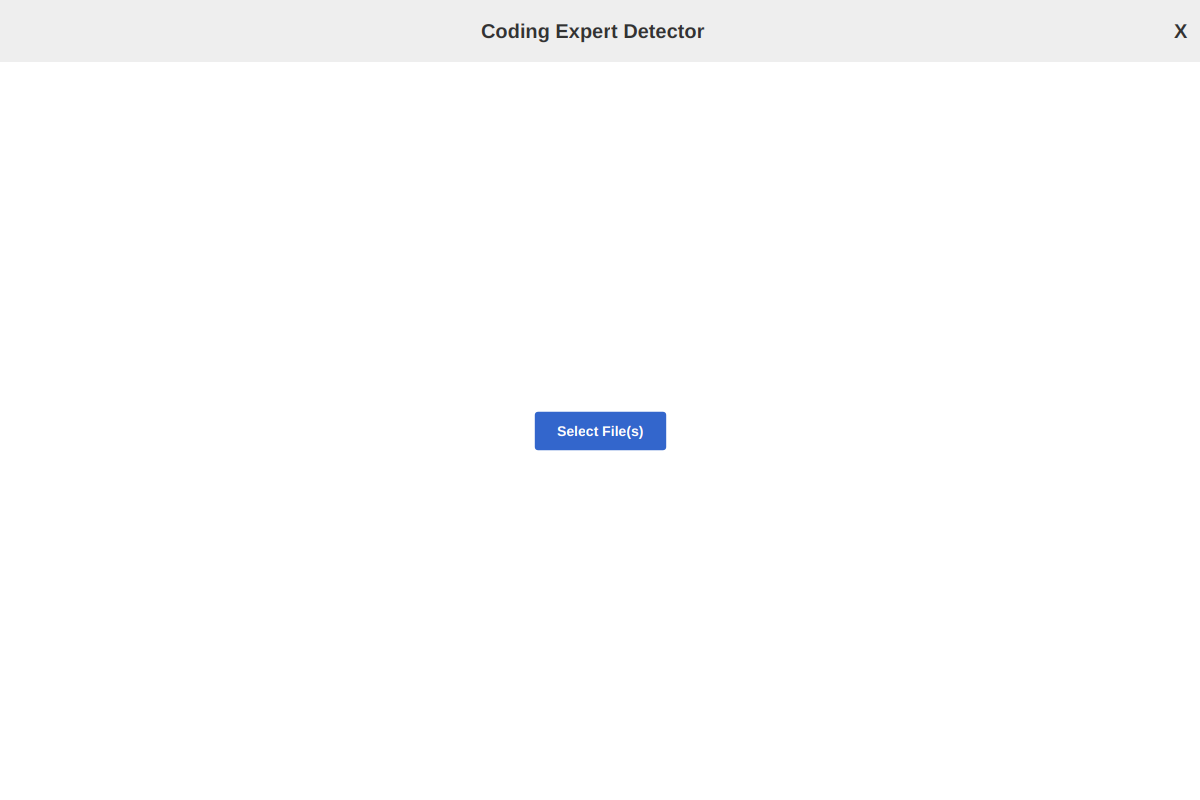
\includegraphics[width=0.8\textwidth]{figure4.9.png}
\caption{Screenshot of the results page, featuring the box plots next to the feature values}
\end{figure}

Back to the point where the array p in the question is 1-based. One alternative solution was to change the array to 0-based in the question and the provided test cases. This was not chosen as the solution as the aim was to keep the question as close as possible to that used in the dataset. Ideally, the entire environment should be made identical to that from the original dataset, to minimize any systematic deviation caused in the evaluation. Changing the array to 0-based would affect how developers solve the question, such as requiring or allowing them to remove, or add, a few more lines as a result of the change. This is not desirable and therefore this solution was not implemented.

Another suggestion received was to provide on-site testing. This feature would allow the user to directly code using the code editor on the webpage and have their code run against test cases through the web interface, removing the need for a user to download and run files locally. This was not implemented due to time constraints. However, it was determined that it would be beneficial to the user experience and if such a site is to be used, this feature would be valuable.

\subsection{Testing}

During the development process, a list of tests has been conducted to ensure the completeness and readiness of the website application. Table 4.2 shows the list, grouped by the type of test conducted, along with the final status of each test.

\begin{longtable}[h!]{m{23em}|m{13em}}
\hline
Test & Results \\
\endhead
\hline
\multicolumn{2}{c}{Functional Tests} \\
\hline
Links in the navigation bar on all pages directs the user to respective pages & Success \\
\hline
Both links to the application page at the homepage directs the user to the application page & Success \\
\hline
Dark and light mode switch toggles the colour scheme to the respective mode on all pages & Success \\
\hline
Both Solution.java and Test.java files can be downloaded through the link on the application page & Success \\
\hline
User can select one, and only one, file in the application through the file selector & Success \\
\hline
The code viewer shows the content of the file selected upon selection & Success \\
\hline
The system rejects submission without a file being selected, showing an error message & Success \\
\hline
The system shows a custom error page for errors triggered, such as by a syntax error in the file submitted & Success \\
\hline
For syntax errors, the system shows debug text of the error & Success \\
\hline
The result page shows a classification of either novice or expert & Success \\
\hline
\multicolumn{2}{c}{Usability Tests} \\
\hline
Content on all pages are free of grammar and spelling mistakes & Success \\
\hline
Links on all pages share the same style and is outstanding from other text & Success \\
\hline
Consistent navigation bar visible on all pages & Success \\
\hline
The site satisfies Web Content Accessibility Guideline requirements, tested by WAVE Web Accessibility Evaluation Tool, made by Utah State University & Success, with no regular errors and text contrast errors \\
\hline
Pass all accessibility tests in Lighthouse by Google & Success, with a 100/100 score \\
\hline
\multicolumn{2}{c}{Compatibility Tests} \\
\hline
All pages display and function properly in IE11, Google Chrome 50, 60, 70, 86, Firefox 60, 70, 82, Opera 50, 60, 71 & Success \\
\hline
All pages display and function properly in any display dimension wider than 300 pixels and taller than 200 pixels & Success \\
\hline
\multicolumn{2}{c}{Performance Tests} \\
\hline
Obtain a score higher than 80/100 in PageSpeed Insights by Google on both mobile and desktop tests & Success, with 87/100 and 98/100 for mobile and desktop tests respectively \\
\hline
Obtain an A grade in GTmetrix’s performance test & Success, obtaining an A grade with 100\% in performance and 95\% in structure tests \\
\hline
\caption{List of tests conducted against the website application, grouped into categories, along with the test results}
\label{tab:4.2}
\end{longtable}

\section{Desktop Application}

\subsection{Design and Implementation}

Another minor prototype created was a desktop application, allowing developer experience classification against multiple files at a time. This application targets group or corporate users. This is a very rough prototype, created with the sole purpose of demonstrating a possible use of the model for group or corporate users.

Implemented with Java using JavaFX, the application only has 2 screens. The first, as shown in Figure 4.10 is one that shows a file selection button, allowing the user to select one or more files to be analyzed. The second, as shown in Figure 4.11, shows the received file’s names, their author experience classification, as well as the features extracted as a table.

\begin{figure}[h!]
\centering
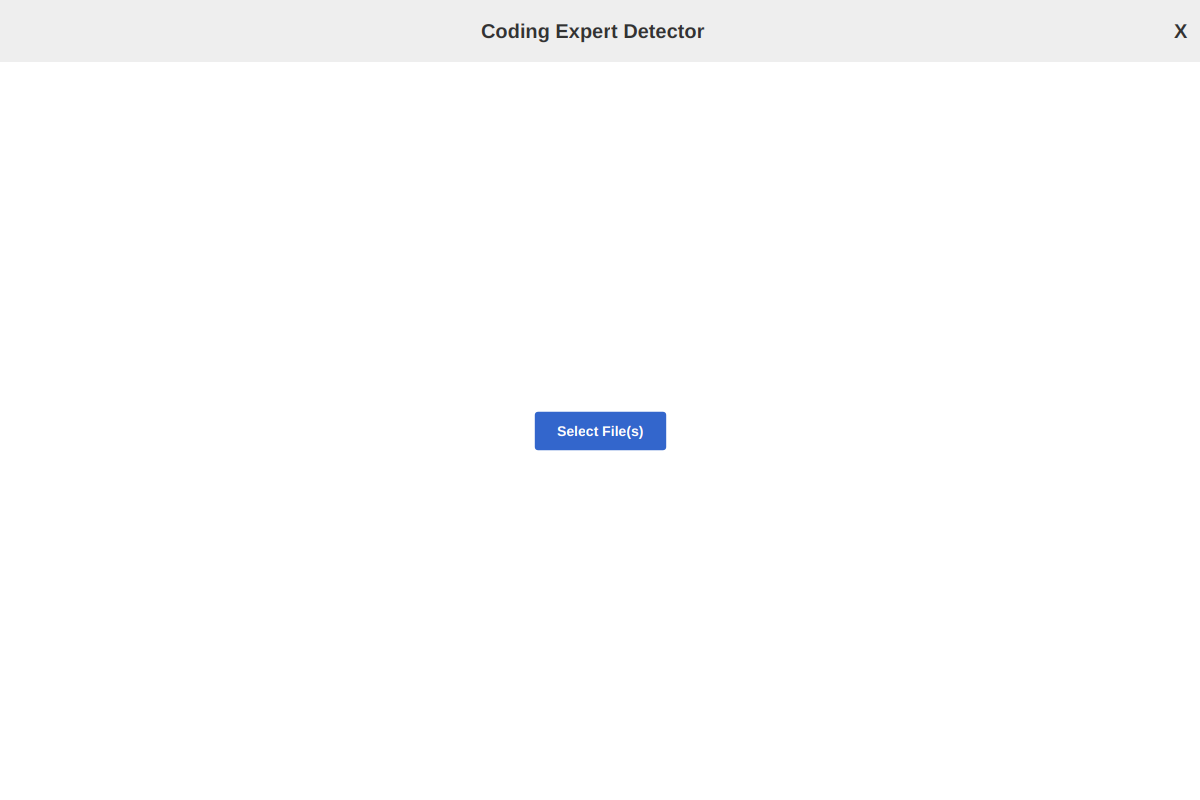
\includegraphics[width=0.8\textwidth]{figure4.10.png}
\caption{Screenshot of the home screen of the desktop application prototype}
\end{figure}

\begin{figure}[h!]
\centering
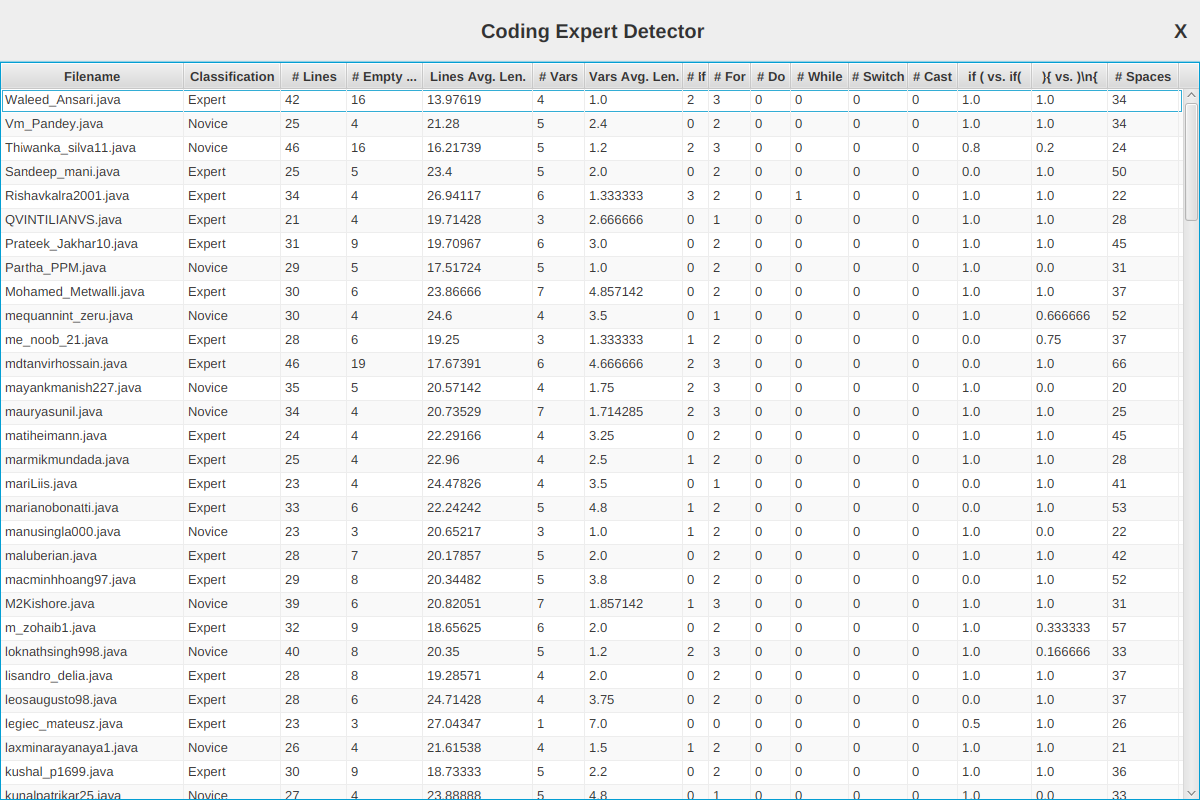
\includegraphics[width=0.8\textwidth]{figure4.11.png}
\caption{Screenshot of the results screen of the desktop application prototype}
\end{figure}

The model itself is not stored in the application. The application was implemented to make a request to the website application’s server to fetch the features extracted and classification results. While this method is not ideal, as it requires an internet connection to connect with the website application’s server and lowers the efficiency of the application as it has to send the request and wait for a reply, it was implemented by exporting a Python model to be used in a Java application could induce unforeseen complications. It should be noted here that with enough study in place for such a solution, it would be more preferable to the current solution.

\subsection{Ethical Concerns}

Given that the application is designed to give corporations the ability to determine one’s programming experience by analyzing their code, ethical concerns may arise regarding related issues.

The preselection of job application candidates would be the biggest concern of all concerns. While it is understood that such pre-selection methods are not always accurate and causes the loss of talents or results in hiring candidates who are not suitable for the job, it could be arguable that these methods help save time for both the company and the candidates, making the entire application process more efficient.

The true concern is if the pre-selection method is fair. As the model was trained using a dataset, biases could be existing in the dataset and be carried over to the final model during the training model. These biases could be due to the bias in the data source itself, or by human-induced, or systematic bias during the collection of data. These biases could damage the reliability of the model, as well as its fairness as it could give an advantage or disadvantage to a group of people whose code exhibits features picked up by the model but non-related to their development experience.

The model developed in this project is not ready for real-life deployment. Not only does it have low accuracy, but it was not thoroughly studied as well, such as to establish the fact that whether there are biases in the model. Before these concerns are investigated and addressed, such a system should not be deployed.

\chapter{Discussions and Conclusion}

\section{Review of Project Aims}

As listed in Section 1.3, a list of 4 aims were set at the beginning of the project. In this section, the completion status of each of those aims, along with discussions regarding the work done will be covered.

\subsection{“Determine if it is possible to classify developers’ experience level using features from their code”}

The first part of this chapter, mainly described in Chapter 3 provides an overview of work done on training a model to classify developers’ experience level using features from their code. The data source, steps for feature extraction, the method for model evaluation, models to train, et cetera were experimented with and discussed. With a 69.0\% accuracy in the final model produced in this project, trained using an extremely focused and limited dataset, it set a baseline for future research into similar topics.

\subsection{“Determine what features would be helpful for the model”}

With the several experiments conducted, along with the analysis of the final model, it was concluded that certain features are more positively linked to novice developers’ behaviours and vice versa. These experiments also helped identify features that affect the model’s accuracy, positively or negatively. These findings were shown in Section 3.4.5

\subsection{“Determine what model would help achieve better classification accuracy”}

Throughout all experiments, a wide set of models were tested and evaluated using their accuracy, as listed in Section 3.3. This helped identify the best performing model, logistic regression, for the dataset.

While there was much work that could be done to further improve different aspects in the whole machine learning model training process, as to be discussed in Section 5.3 Future Work, it could be said that the aims set out related to the model is fulfilled.

\subsection{“Develop one or more prototype applications to demonstrate possible uses of such model”}

As the main focus of Chapter 4, 2 applications were developed. One developed as a website application utilizing the trained model, completed with full user interface design, testing and feedback evaluation, and another application developed as a desktop application prototype, mostly for demonstration purposes.

The aim set is completed, with the website application fully developed. However, it would have been a bigger success if similar could be said about the desktop application. Further work that could be done regarding the applications will be discussed in Section 5.3.

\section{Limitations}

There were two main limitations restricting the progress of the project, namely time constraints and the lack of knowledge, as discussed below. These limitations gave the project much space for future improvements.

Time-wise, this project has very limited time, 20 weeks, for its completion, including the planning and report-writing processes. Many decisions made, such as not to do further experiments on the development of the model, or not complete the desktop application development, were hugely affected by the time constraint.

Knowledge-wise, having a little more than 2 years of background studying in a computer science bachelor degree, also restricted some possibilities of the project, together with the time limitations. Not having any rich knowledge or industry experience in topics such as code stylometry and machine learning, quite a lot of time had to be spent on research. Besides, this inevitably also affects the quality of the work, by not using industry or academic standard methods to conduct certain tasks, such as to measure the accuracy of the models. Although doing all the background research as mentioned in Chapter 2 did provide certain vital information and techniques for this project, many things had to be discovered and learnt in practice.

\section{Future Work}

With the limitations mentioned in the previous section, there are many things in the project that could be improved or further worked on, which will be discussed in this section.

\subsection{A More General and Larger Dataset}

The current dataset is very specific, all short Java solutions to the same coding question. The specificity was desirable for this project as it helps narrow the scope of the project, possibly saving time. However, to make a bigger impact in the field, the dataset must not be so limited and should be generalized, such that more types of code could be analyzed. Besides, the size of the dataset used in this project was rather small. A larger dataset could benefit the model’s accuracy.

\subsection{Experiments on Features}

In this project, several experiments were carried on testing different features to be extracted from the code samples to evaluate their effectiveness in improving the accuracy of the models being trained. However, most of those features were more simple ones, such that they are easily extracted and the values are mostly directly used in the dataset without any organization or preprocessing. More experiments could be carried on more complex features, such as n-grams and more abstract syntax tree features, as well as to test different combinations of those features against the accuracy of the models.

\subsection{Experiments on Models}

Besides features extraction, another important part of this project is the set of models to be trained. While the set of models selected for this project is rather diverse, representing a wide range of types of model, there were no adjustments or configurations made on those models. Further work could be done to experiment with different configurations of those models, or to test new models of the same type as the best models from the existing group, in an attempt to reach better results.

\subsection{Study on Models}

More work could also be done on the final model, where the correlation found between features and the classification could be further studied, as well as to test the model in extreme cases and against possible biases cases.

\subsection{Further Application Development}

For the website application, a larger user test and evaluation could be beneficial to collect more ideas for improving the site. It is also worth holding ethical discussions before publishing the site for individual uses, once a good model is ready for it.

For the desktop application, future works could complete the existing prototype or take the existing prototype as an example to develop a program with similar features for the same target user group, which in this case is for group or corporate users.

\subsection{Publish Research}

Last but not the least, is to publish the findings of this project, mainly the machine learning model part, and best with the addition of possible future works done. While there were no new trivial approaches to training a model or new method for dataset construction, it is believed that the value of this project is that it explores the possibility of using the machine learning approach to categorize developers according to their development experience, which is undone, and provides a base for any futures studies in this field, which could possible bring a huge impact to the internet technology industry.

\section{Personal Remarks}

In this section, personal remarks will be covered, in a less formal format than other chapters.

To conclude this project, I would say that it was a success, at least technically a success, as all the aims we set at the beginning of the project were fully completed. Looking at the final products, a 69.0\% accurate model, a fully developed web application and a desktop application prototype, many things could have been done better, such as those discussed in Section 5.3 Future Work, to achieve better results. However, regrettably, this was not possible given the time constraint. While a 69.0\% accuracy is not bad at all, especially for a bachelor student in a 20-week project, I believe it could be much better with more time and resources spent in the research. I would not say that the project was a great success, but I am still very thankful for the completion of this amazing project, which I truly believe does possibly have great value.

Most techniques or processes used in this project are self-learnt, if one would like to know how much I’ve learnt in this project. Although I view this project as an amateur academic research, I do understand that the School of Computing and Communications view this as a student project and therefore would like students to state how much they have learnt, which therefore is listed below:

\begin{itemize}
\item Machine learning dataset collection and construction techniques
\item Machine learning model training and analysis techniques
\item Machine learning results handling and presentation techniques
\item Application development process
\end{itemize}

The biggest thing that I’ve got out of these 20 weeks, in my opinion, is not any of the above knowledge, but rather the experience of conducting a study in the computer science field. I have had experience with biotechnology research studies but never a computer science research. This project gave me the rare experience of conducting research independently with a supervisor from the planning process, to execution. Throughout the process, I have learnt to appreciate certain practices academics use, such as their data presentation techniques, as well as the importance of citing in writings, et cetera.

I would like to once again thank this project’s supervisor, Professor Tracy Hall for her guidance, support and feedback along the way.

Finally, although there are certain regrets regarding some limitations of the project, I would say that this was a good project, achieving great results overall and I enjoyed it a lot. I am hopeful that more studies would be conducted into this field as I believe it will bring a positive impact on the technology industry.

\pagenumbering{roman}
\newpage
\addcontentsline{toc}{section}{References}
\begin{center}
    \textbf{References}
\end{center}
(ordered alphabetically)

Agrawal, R., Golshan, B. and Terzi, E. (2014). Grouping students in educational settings. \textit{Proceedings of the 20th ACM SIGKDD international conference on Knowledge discovery and data mining - KDD ’14}. 10.1145/2623330.2623748

Alsulami, B., Dauber, E., Harang, R., Mancoridis, S. and Greenstadt, R. (2017). Source Code Authorship Attribution Using Long Short-Term Memory Based Networks. \textit{Computer Security – ESORICS 2017}, pp.65–82.

Babcock, P. (2003). \textit{Spotting Lies}. [online] SHRM. Available at: https://www.shrm.org/hr-today/news/hr-magazine/pages/1003babcock.aspx [Accessed 13 Feb. 2021].

Bhattathiripad, P.V. (2012). Software Piracy Forensics: A Proposal for Incorporating Dead Codes and Other Programming Blunders as Important Evidence in AFC Test. \textit{2012 IEEE 36th Annual Computer Software and Applications Conference Workshops}.

Burrows, S. and Tahaghoghi, S.M.M. (2007). Source code authorship attribution using n-grams. \textit{Proceedings of the Twelfth Australasian Document Computing Symposium, Melbourne, Australia, RMIT University}, pp.32–39.

Caliskan-Islam, A., Harang, R., Liu, A., Narayanan, A., Voss, C., Yamaguchi, F. and Greenstadt, R. (2015). De-anonymizing Programmers via Code Stylometry. \textit{Proceedings of the 24th USENIX Security Symposium}, pp.255–270.

Castellanos, H., Restrepo-Calle, F., Gonzalez, F.A. and Echeverry, J.J.R. (2017). Understanding the relationships between self-regulated learning and students source code in a computer programming course. \textit{2017 IEEE Frontiers in Education Conference (FIE)}.

Clark, J.G., Walz, D.B. and Wynekoop, J.L. (2003) Identifying Exceptional Application Software Developers: A Comparison of Students and Professionals. \textit{Communications of the Association for Information Systems}, 11, 137-154. 10.17705/1CAIS.01108

Counsell, S., Swift, S., Tucker, A. and Mendes, E. (2006). Object-oriented cohesion subjectivity amongst experienced and novice developers. \textit{ACM SIGSOFT Software Engineering Notes}, 31(5), pp.1–10.

Google Code Jam. (2021). \textit{Code Jam - Google’s Coding Competitions}. [online] Available at: https://codingcompetitions.withgoogle.com/codejam [Accessed 26 Feb. 2021].

Guillen-Nieto, V., Vargas Sierra, C., Pardino-Juan, M., Martinez-Barco, P. and Suarez-Cueto, A. (2008). Exploring State-of-the-Art Software for Forensic Authorship Identification. \textit{International Journal of English Studies}, 8(1), pp.1–28.

HackerRank (2021). \textit{About Us}. [online] HackerRank. Available at: https://www.hackerrank.com/about-us [Accessed 2 Mar. 2021].

Halstead, M.H. (1977). \textit{Elements of software science (operating and programming systems series)}. Elsevier Science Inc.

Hayes, J.H. and Offutt, J. (2010). Recognizing authors: an examination of the consistent programmer hypothesis. \textit{Software Testing, Verification and Reliability}, 20(4), pp.329–356.

JavaParser (2021). \textit{JavaParser - Home}. [online] javaparser.org. Available at: https://javaparser.org/.

Jha, A., Chandrasekaran, A., Kim, C. and Ramprasad, R. (2019). Impact of dataset uncertainties on machine learning model predictions: the example of polymer glass transition temperatures. \textit{Modelling and Simulation in Materials Science and Engineering}, 27(2), p.024002.

Job Today. (2017). \textit{One in Three UK Jobseekers Lie on their CV}. [online] Available at: https://jobtoday.com/gb/blog/one-four-uk-jobseekers-lie-cv/ [Accessed 13 Feb. 2021].

Kalgutkar, V., Kaur, R., Gonzalez, H., Stakhanova, N. and Matyukhina, A. (2019). Code Authorship Attribution. \textit{ACM Computing Surveys}, 52(1), pp.1–36.

Krsul, I. and Spafford, E.H. (1997). Authorship analysis: identifying the author of a program. \textit{Computers \& Security}, 16(3), pp.233–257.

Loksa, D., Ko, A.J., Jernigan, W., Oleson, A., Mendez, C.J. and Burnett, M.M. (2016). Programming, Problem Solving, and Self-Awareness. \textit{Proceedings of the 2016 CHI Conference on Human Factors in Computing Systems}.

Lui, A.K., Kwan, R., Poon, M. and Cheung, Y.H.Y. (2004). Saving weak programming students. \textit{ACM SIGCSE Bulletin}, 36(2), p.72.‌ 10.1145/1024338.1024376

Mori, T. and Uchihira, N. (2018). Balancing the trade-off between accuracy and interpretability in software defect prediction. \textit{Empirical Software Engineering}, 24(2), pp.779–825.

Oman, P.W. and Cook, C.R. (1989). Programming style authorship analysis. \textit{Proceedings of the seventeenth annual ACM conference on Computer science: Computing trends in the 1990’s Computing trends in the 1990’s - CSC ’89}.

Patricia, S. (2014). The Impact of the Self-Awareness Process on Learning and Leading. \textit{New England Journal of Higher Education}.

Platt, J.C. (1998). Sequential Minimal Optimization: A Fast Algorithm for Training Support Vector Machines.

Shevertalov, M., Kothari, J., Stehle, E. and Mancoridis, S. (2009). On the Use of Discretized Source Code Metrics for Author Identification. \textit{2009 1st International Symposium on Search Based Software Engineering}.

Simko, L., Zettlemoyer, L. and Kohno, T. (2018). Recognizing and Imitating Programmer Style: Adversaries in Program Authorship Attribution. \textit{Proceedings on Privacy Enhancing Technologies}, 2018(1), pp.127–144.

Therrien, R. and Doyle, S. (2018). Role of training data variability on classifier performance and generalizability. \textit{Medical Imaging 2018: Digital Pathology}, 10581.

Thunes, C. (2021). \textit{c2nes/javalang}. [online] GitHub. Available at: https://github.com/c2nes/javalang [Accessed 8 Mar. 2021].

Violentmonkey (2021). \textit{Violentmonkey}. [online] Violentmonkey. Available at: https://violentmonkey.github.io/ [Accessed 8 Mar. 2021].

Virtual Machinery (2021). \textit{JHawk - the Java metrics tool - Product Overview}. [online] www.virtualmachinery.com. Available at: http://www.virtualmachinery.com/jhawkprod.htm [Accessed 13 Mar. 2021].

Wiedenbeck, S. (1985). Novice/expert differences in programming skills. \textit{International Journal of Man-Machine Studies}, 23(4), pp.383–390.

Wisse, W. and Veenman, C. (2015). Scripting DNA: Identifying the JavaScript programmer. \textit{Digital Investigation}, 15, pp.61–71.

Zhang, C., Wang, S., Wu, J. and Niu, Z. (2017). Authorship Identification of Source Codes. \textit{Web and Big Data}, pp.282–296.

\newpage
\addcontentsline{toc}{section}{Appendix}
\begin{center}
    \textbf{Appendix}
\end{center}

\addcontentsline{toc}{subsection}{Original Project Proposal}
\begin{center}
    \textbf{Original Project Proposal}
\end{center}

\includepdf[pages=-, width=1.2\textwidth, frame]{proposal.pdf}

\addcontentsline{toc}{subsection}{List of Significant Experiments}
\begin{center}
    \textbf{List of Significant Experiments}
\end{center}

\begin{longtable}[h!]{m{4.5em}m{2.5em}m{3em}m{3em}m{18em}}
\hline
Experiment ID & Week \# & Meeting \# & \# of Rows & Details \\
\hline
\endhead
1 & 4 & 6 & 27 & Any work experience = experienced \\
2 & 4 & 6 & 106 & 6 months after first job = experienced; 6 months before first job/intern = novice, new data used because of new work experience definition and slight difference in data collection process \\
3 & 4 & 6 & 174 & 2 with more new data \\
16 & 6 & 8 & 266 & Without complexity, With general code \\
17 & 6 & 8 & 266 & Without complexity, Without general code \\
18 & 6 & 8 & 266 & With complexity, With general code \\
19 & 6 & 8 & 266 & With complexity, Without general code \\
20 & 7 & 9 & 266 & 16 with Halstead metrics \\
21 & 7 & 9 & 266 & 17 with Halstead metrics \\
22 & 7 & 9 & 266 & 18 with Halstead metrics \\
23 & 7 & 9 & 266 & 19 with Halstead metrics \\
24 & 7 & 9 & 157 & 19 with only JHawk metrics \\
25 & 7 & 9 & 157 & 19 combined with JHawk metrics \\
26 & 6 & 8 & 196 & Regression Test \\
27 & 8 & 10 & Variable & 19 dataset split by questions \\
28 & 8 & 10 & 83 & Based on 19, with more solutions for the question: Kangaroo (50 -> 83) \\
29 & 8 & 10 & 51 & Based on 19, with more solutions for the question: Grading (27 -> 51) \\
31 & 9 & 11 & 55 & Question: Circular Array Rotation, 55 rows (new), original \\
32 & 9 & 11 & 55 & Question: Circular Array Rotation, 55 rows (new), no general \\
33 & 9 & 11 & 79 & Question: Circular Array Rotation, 79 rows (new + old 55), original \\
34 & 9 & 11 & 79 & Question: Circular Array Rotation, 79 rows (new + old 55), no general \\
35 & 11 & 13 & 69 & Question: Sequence Equation, 69 rows, original \\
36 & 11 & 13 & 69 & Question: Sequence Equation, 69 rows, original, no general \\
37 & 11 & 13 & 90 & Question: Sequence Equation, 90 rows (inc'l old 69), original \\
38 & 11 & 13 & 90 & Question: Sequence Equation, 90 rows (inc'l old 69), original, no general \\
39 & 11 & 13 & 164 & Question: Sequence Equation, all new users parsed using script, original \\
40 & 11 & 13 & 164 & Question: Sequence Equation, all new users parsed using script, no general \\
41 & 19 & 20 & 164 & Set 40, with min max scaler \\
42 & 19 & 20 & 164 & Set 40, with standard scaler \\
\hline
\end{longtable}

\setlength{\parskip}{0.5em}

\addcontentsline{toc}{subsection}{List of Figures}
\listoffigures

\addcontentsline{toc}{subsection}{List of Tables}
\listoftables

\end{document}

